
% VLDB template version of 2020-08-03 enhances the ACM template, version 1.7.0:
% https://www.acm.org/publications/proceedings-template
% The ACM Latex guide provides further information about the ACM template

%\documentclass[sigconf, nonacm]{acmart}
\documentclass[sigconf, anonymous]{acmart} % replace this with the one above for the camera-ready


\usepackage{algorithm}
\usepackage{algpseudocode}
\usepackage{subcaption}
\usepackage{placeins}
\usepackage{diagbox}
\usepackage{array}
\usepackage[table]{xcolor}  % For coloring
\usepackage{booktabs}
\usepackage{caption}
\usepackage[utf8]{inputenc}
\usepackage{tikz}
\usepackage[symbol]{footmisc}
\usepackage{float}
\usepackage{needspace}
\usepackage{enumitem}
\usetikzlibrary{shapes.geometric, arrows.meta, positioning, calc, patterns}

\setlength{\abovecaptionskip}{3pt}
\setlength{\belowcaptionskip}{3pt}

%% The following content must be adapted for the final version
% paper-specific
\newcommand\vldbdoi{XX.XX/XXX.XX}
\newcommand\vldbpages{XXX-XXX}
% issue-specific
\newcommand\vldbvolume{14}
\newcommand\vldbissue{1}
\newcommand\vldbyear{2020}
% should be fine as it is
\newcommand\vldbauthors{\authors}
\newcommand\vldbtitle{\shorttitle} 
% leave empty if no availability url should be set
\newcommand\vldbavailabilityurl{URL_TO_YOUR_ARTIFACTS}
% whether page numbers should be shown or not, use 'plain' for review versions, 'empty' for camera ready
\newcommand\vldbpagestyle{plain} 

\settopmatter{authorsperrow=3}

\begin{document}
\title{QVCache: A Query-Aware Vector Cache}

%%
%% The "author" command and its associated commands are used to define the authors and their affiliations.
\author{Anıl Eren Göçer}
\affiliation{%
  \institution{ETH Zurich}
  \city{Zurich}
  \state{Switzerland}
}
\email{agoecer@ethz.ch}

\author{Ioanna Tsakalidou}
\affiliation{%
  \institution{EPFL}
  \city{Lausanne}
  \state{Switzerland}
}
\email{ioanna.tsakalidou@epfl.ch}

\author{Hamish Nicholson}
\affiliation{%
  \institution{EPFL}
  \city{Lausanne}
  \state{Switzerland}
}
\email{hamish.nicholson@epfl.ch}

\author{Kyoungmin Kim}
\affiliation{%
  \institution{EPFL}
  \city{Lausanne}
  \state{Switzerland}
}
\email{kyoung-min.kim@epfl.ch}

\author{Anastasia Ailamaki}
\affiliation{%
  \institution{EPFL}
  \city{Lausanne}
  \state{Switzerland}
}
\email{anastasia.ailamaki@epfl.ch}

%%
%% The abstract is a short summary of the work to be presented in the
%% article.

\begin{abstract}
Vector databases have become a cornerstone of modern information retrieval, powering applications in recommendation, search, and retrieval-augmented generation (RAG) pipelines. However, scaling Approximate Nearest Neighbor (ANN) search to high recall under strict latency SLOs remains fundamentally constrained by memory capacity and I/O bandwidth. Disk-based vector search systems suffer severe latency degradation at high accuracy, while fully in-memory solutions incur prohibitive memory costs at billion-scale. Despite the central role of caching in traditional databases, vector search lacks a general query-level caching layer capable of amortizing repeated query work.

We present QVCache, the first backend-agnostic query-level caching system for ANN search with bounded memory footprint. QVCache exploits semantic query repetition by performing similarity-aware caching rather than exact-match lookup. It dynamically learns region-specific distance thresholds using an online learning algorithm, enabling recall-preserving cache hits while bounding lookup latency and memory usage independently of dataset size. QVCache operates as a drop-in layer for existing vector databases. It maintains a megabyte-scale memory footprint and achieves sub-millisecond cache-hit latency, reducing end-to-end query latency by up to 40–1000× when integrated with existing ANN systems. For workloads exhibiting temporal-semantic locality, QVCache substantially reduces latency while preserving recall comparable to the underlying ANN backend, establishing it as a missing but essential caching layer for scalable vector search.
\end{abstract}

\begin{comment}
    Vector databases have become a cornerstone of modern information retrieval, powering applications in recommendation, search, and retrieval-augmented generation (RAG) pipelines. While caching is a well-studied problem in traditional databases, a dedicated caching layer is absent in the vector search literature. Disk-based vector search suffers from high latencies in high-accuracy settings, whereas fully in-memory solutions cannot scale to billion-scale datasets. We present QVCache, the first backend-agnostic vector search cache designed to fill this gap, capable of working with any existing vector database. QVCache delivers sub-millisecond query latencies, achieving up to 300$\times$ lower latency on a cache hit compared to disk-based vector databases for billion-scale datasets. It uses only a megabyte-scale memory footprint by keeping in memory a very small hot set of vectors regardless of dataset size, which is negligible compared to fully in-memory systems for practical workloads. Unlike conventional caches, QVCache addresses the unique challenge of similarity caching, where cache hits cannot be determined by exact key matches. It solves this problem by applying an online learning algorithm that dynamically adjusts spatial distance thresholds governing cache hit decisions and keeps the cache size bounded through an eviction policy. QVCache is particularly effective for workloads exhibiting temporal-semantic locality, achieving orders of magnitude lower latencies on cache hits while maintaining recall comparable to that of the backend database. Our results establish QVCache as a missing but crucial caching layer for efficient large-scale similarity search.
\end{comment}

\maketitle

%%% do not modify the following VLDB block %%
%%% VLDB block start %%%
\pagestyle{\vldbpagestyle}
\begingroup\small\noindent\raggedright\textbf{PVLDB Reference Format:}\\
\vldbauthors. \vldbtitle. PVLDB, \vldbvolume(\vldbissue): \vldbpages, \vldbyear.\\
\href{https://doi.org/\vldbdoi}{doi:\vldbdoi}
\endgroup
\begingroup
\renewcommand\thefootnote{}\footnote{\noindent
This work is licensed under the Creative Commons BY-NC-ND 4.0 International License. Visit \url{https://creativecommons.org/licenses/by-nc-nd/4.0/} to view a copy of this license. For any use beyond those covered by this license, obtain permission by emailing \href{mailto:info@vldb.org}{info@vldb.org}. Copyright is held by the owner/author(s). Publication rights licensed to the VLDB Endowment. \\
\raggedright Proceedings of the VLDB Endowment, Vol. \vldbvolume, No. \vldbissue\ %
ISSN 2150-8097. \\
\href{https://doi.org/\vldbdoi}{doi:\vldbdoi} \\
}\addtocounter{footnote}{-1}\endgroup
%%% VLDB block end %%%

%%% do not modify the following VLDB block %%
%%% VLDB block start %%%
\ifdefempty{\vldbavailabilityurl}{}{
\vspace{.3cm}
\begingroup\small\noindent\raggedright\textbf{PVLDB Artifact Availability:}\\
The source code, data, and/or other artifacts have been made available at \url{\vldbavailabilityurl}.
\endgroup
}
%%% VLDB block end %%%

\section{Introduction}
%Needs to answer:
%1)necessity, whats the problem
%2)impact of the solution
%3)applicability to today's issues

% introduce the topic
Modern data-intensive services increasingly rely on Approximate Nearest Neighbor (ANN) search over high-dimensional embeddings. However, scaling ANN to high recall under strict latency SLOs remains fundamentally constrained by memory capacity and I/O bandwidth.
This tension is now a dominant systems bottleneck: improving recall predictably inflates latency and operational cost, while controlling latency requires either aggressive approximation or prohibitively large memory footprints. As a result, ANN has become a first-order performance and cost concern in production systems, including recommendation pipelines~\cite{Covington:2016:DNN:YouTube}, search engines~\cite{Liu:2021:Q2S:Facebook, amazon-shop-the-look, visrel}, and Retrieval-Augmented Generation (RAG) workloads for large language models (LLMs)~\cite{Lewis:2020:RAG:NeurIPS, gao2024retrievalaugmentedgenerationlargelanguage}. 

% the problem
This bottleneck is structural rather than incidental. Achieving high recall in ANN search requires traversing increasingly large and irregular neighborhoods in high-dimensional space, leading to random access amplification that cannot be efficiently prefetched or batched. In graph- and quantization-based indexes, recall improvements translate directly into expanded graph exploration, candidate explosion, and deeper disk or memory accesses. 
%Importantly, this tradeoff is not specific to a particular index structure: graph-based, quantization-based, and tree-based ANN indexes all incur increasing random access as recall increases. 
Although in-memory ANN systems achieve low latency, their memory cost grows linearly with the size of the dataset. Disk-based systems reduce memory pressure, but suffer severe latency degradation at high recall and large result sets $k$, where pointer chasing and random I/O dominate execution time. As a result, operators are forced into an undesirable choice between cost and performance, with no mechanism to amortize repeated query work over time.

% enabler
A natural response to repeated expensive computation is caching. Across the systems stack, caching has been the primary mechanism for amortizing work, from hardware memory hierarchies~\cite{memory-hierarchy} to database buffer pools~\cite{dbmin,data-caching-for-enterprise-scale}, intermediate results caching~\cite{caching-intermediate-results}, and final query result caches~\cite{memcached,redis2025}. These techniques rely on a core assumption: identical queries recur. This assumption underlies the cache abstraction itself, which treats queries as discrete keys rather than points in a metric space. However, in vector search, this assumption is invalid. Even minor changes in user inputs or prompts produce distinct embeddings, making exact-match caching ineffective~\cite{Covington:2016:DNN:YouTube, gao2024retrievalaugmentedgenerationlargelanguage}. Consequently, ANN systems effectively forfeit one of the most powerful tools in the systems toolbox.

% solutions so far
Existing ANN systems rely on index-internal heuristics—such as caching centroids~\cite{diskann} or upper graph layers~\cite{tiered-cache-hnsw}—to reduce average I/O. These mechanisms reduce constant factors but cannot eliminate backend execution, cannot exploit workload locality at the query level, and cannot generalize across ANN backends. Consequently, operators are forced into a persistent tradeoff between memory cost and latency, with no mechanism to amortize query work across time.

% insight
The key insight of this work is that query repetition in vector search is semantic rather than exact. Real workloads exhibit temporal locality in embedding space: while query vectors are rarely identical, they are often sufficiently close that their nearest-neighbor sets are interchangeable at target recall. Exploiting this locality requires treating caching as a similarity problem rather than an exact lookup problem~\cite{similarity-caching}. However, similarity caching in high-dimensional vector spaces introduces two unresolved systems challenges: (1) selecting similarity thresholds that preserve recall without collapsing hit rates, and (2) performing cache lookups efficiently without turning the cache itself into a nearest neighbor index with unbounded latency and memory growth. Naively addressing either challenge leads to unbounded false positives that lower recall, or to cache designs whose overhead rivals the backend ANN system.

Prior work on similarity caching provides theoretical foundations but does not address the constraints of ANN serving systems~\cite{similarity-caching,similarity-caching-theory-algorithms}. Existing practical systems for LLM response caching rely on fixed global thresholds~\cite{gptcache}, which perform poorly under heterogeneous query distributions, or tightly couple caching logic to a specific index structure~\cite{vcache}. None provide a general, query-level cache that is backend-agnostic, recall-aware, and resource-bounded.

% our solution
We introduce \textbf{QVCache}, a new caching system for ANN search: a similarity-aware, recall-preserving query cache with fixed resource budgets. 
%Unlike traditional caches that map discrete keys to results, QVCache maps regions of the embedding space to recall-valid nearest-neighbor sets.
QVCache assigns region-specific similarity thresholds in the embedding space and dynamically adapts them using an online learning algorithm driven by observed nearest-neighbor distance statistics. This design bounds lookup latency and memory usage independently of dataset size, while aggressively short-circuiting backend ANN queries without compromising recall.

% impact of the solution
QVCache is designed as a drop-in layer for existing ANN systems. It requires no changes to index construction, applies uniformly to in-memory and disk-based backends. Unlike ANN indexes, QVCache does not grow with dataset size, does not aim for asymptotic recall completeness, and never replaces backend search on cache misses. By converting semantic locality into amortized query execution, QVCache reduces backend load and latency in high-recall settings without increasing memory pressure. This allows meeting latency SLOs at high recall without provisioning fully in-memory ANN indexes.

% contributions
The contributions of this paper are:
\begin{itemize}
    \item A formulation of query-level vector caching as a similarity-aware, recall-constrained systems problem.

    \item The design of QVCache, a backend-agnostic ANN cache with adaptive, region-specific similarity thresholds and bounded latency and memory, which we show can reduce end-to-end latency by up to \(40\text{–}1000\times\) when integrated with existing ANN systems, while maintaining a memory footprint typically below 1\% of fully in-memory indexes.

    \item An online threshold-learning algorithm driven by observed nearest-neighbor distance statistics.

    \item A workload generation benchmarking framework for controlled temporal-semantic locality in vector search, enabling reproducible evaluation of vector caching systems.
\end{itemize}

\begin{comment}

Approximate Nearest Neighbor (ANN) search is a core primitive in modern data-intensive systems, underpinning applications such as recommendation systems~\cite{Covington:2016:DNN:YouTube}, search engines~\cite{Liu:2021:Q2S:Facebook, amazon-shop-the-look, visrel}, and large language models (LLMs) via Retrieval-Augmented Generation (RAG)~\cite{Lewis:2020:RAG:NeurIPS, gao2024retrievalaugmentedgenerationlargelanguage}. In these systems, user inputs, such as queries or prompts often augmented with contextual information~\cite{task-embeddings-learning-query-embeddings-using-task-context}, are mapped to high-dimensional embeddings using neural models~\cite{devlin2019bertpretrainingdeepbidirectional,mikolov2013efficientestimationwordrepresentations}. These embeddings are designed to preserve semantic similarity, placing related inputs close to one another in a shared vector space. Likewise, system objects, including videos~\cite{Covington:2016:DNN:YouTube}, products~\cite{Liu:2021:Q2S:Facebook}, and documents~\cite{distributed-representations-of-sentences-and-documents}, are represented as vectors in the same space. Answering a query therefore reduces to performing a vector search that retrieves the nearest object vectors to the query embedding. However, serving such vector search queries at scale presents a fundamental tension between memory cost and latency.


Nearest neighbor search is inherently computationally expensive, with a time and space complexity of $O(n \cdot d)$ where $n$ is the number of vectors and $d$ is their dimensionality~\cite{graph-based-vector-search-evaluation}. For this reason, exhaustive search is impractical in most scenarios, particularly for large-scale datasets. Consequently, nearly all vector databases employ various approximation techniques to reduce the number of comparisons~\cite{HNSWMalkovY16,diskann, product-quantization, spann,locality-sensitive-hashing,kd-tree-nn, faiss} and to lower the memory footprint~\cite{product-quantization}.

Due to the approximate nature of nearest neighbor search, there is a fundamental trade-off between search accuracy (recall) and performance (latency and throughput)~\cite{ann-analyses}. Among the various approaches, graph-based indexing methods ~\cite{diskann,HNSWMalkovY16,elpis, nsg} and inverted file indexes (IVF) ~\cite{product-quantization, faiss, spann}    have emerged as the most effective in balancing this trade-off. During index construction, graph-based methods build a proximity graph where each node represents a vector stored in the database, and edges connect vectors that are close to each other in the vector space. During query processing, the search begins from a pre-selected set of entry points and proceeds in a best-first manner until no closer candidate vectors are found ~\cite{graph-based-vector-search-evaluation, diskann, elpis, HNSWMalkovY16, nsg}.
On the other hand, IVF indexes partition the high-dimensional space into multiple regions. During query processing, the partitions closest to the query vector are identified, and similarity comparisons are performed only within those selected partitions.

While some systems store both the index and vectors on disk, primarily SSDs~\cite{diskann,spann,scalablediskbasedapproximatenearest}, others keep them entirely in memory~\cite{faiss}, and some support both options~\cite{milvus,weaviate2025,qdrant2025}, allowing users to select the storage medium for the vectors and index based on factors such as dataset size and performance requirements. In-memory systems have very high memory footprints, which increase substantially with dataset size, even during search, often reaching hundreds of gigabytes for billion-scale datasets~\cite{graph-based-vector-search-evaluation}. In contrast, disk-based systems can operate on commodity machines with tens of gigabytes of memory. However, they suffer from significantly higher latencies in high-recall settings; latency increases while throughput decreases exponentially as recall requirements grow due to excessive random accesses to disk ~\cite{diskann,scalablediskbasedapproximatenearest,parlayann, turbocharging-vector-databases-ssds}. This performance degradation becomes more severe when queries request a larger number of neighbors, as each query triggers exponentially more comparisons and random disk accesses ~\cite{parlayann}.

Over the decades, system researchers have leveraged caching to avoid repeating expensive operations, exploring it at various layers of modern systems, from the hardware stack~\cite{memory-hierarchy} to the application layer~\cite{caching-search-query-results}. This problem is particularly well-studied in databases, which cache pages at the storage layer~\cite{dbmin,data-caching-for-enterprise-scale}, intermediate results~\cite{caching-intermediate-results}, or final query results~\cite{memcached,redis2025}. Despite these efforts, caching in vector search remains largely unexplored~\cite{vdbms-survey-sigmod,vdbms-survey-extensive}. Existing approaches are limited and superficial: for instance, DiskANN~\cite{diskann} stores points near the centroid of the graph to reduce disk accesses during queries, and Tiered Cache-HNSW~\cite{tiered-cache-hnsw} keeps part of the highest layer of HNSW in memory. Both methods are system-level caches embedded within their respective systems, reducing disk access but not eliminating it entirely.

To the best of our knowledge, building a query-level cache for ANN search similar to Redis~\cite{redis2025} or Memcached~\cite{memcached}, which relies on the assumption that queries exhibit temporal locality, has not been attempted. This is a challenging problem in the context of vector search, as it is highly unlikely to receive the \emph{exact same} query vector multiple times. Even small changes in the user query or prompt produce different (but similar) vectors during 
the embedding generation step~\cite{Covington:2016:DNN:YouTube, gao2024retrievalaugmentedgenerationlargelanguage}.

This characteristic makes vector caching a form of the \textit{similarity caching} problem ~\cite{similarity-caching}. Unlike exact caching, similarity caching serves a query $q$ from the cache if it contains an entry for a sufficiently similar query $q'$, i.e., when $d(q, q') < r$, where $r$ is a similarity threshold defined in a metric space~\cite{similarity-caching,similarity-caching-theory-algorithms}. Another instance of similarity caching arises in LLM response caching. For example, GPTCache~\cite{gptcache} employs a static similarity threshold to determine cache hits, whereas vCache~\cite{vcache} highlights the importance of using adaptive thresholds for each cached prompt to optimize hit rates.

We present QVCache, the first query-level vector cache designed to address the unique challenges of similarity caching in vector search. QVCache assigns distinct similarity thresholds to different regions of the high-dimensional vector space and dynamically adjusts these thresholds using an online learning algorithm. It ensures bounded cache hit latency and a bounded memory footprint, independent of the dataset size, through a novel cache eviction strategy. Furthermore, QVCache leverages the distance between a query vector and its furthest nearest neighbor to learn these thresholds, enabling it to achieve a recall close to that of the underlying backend vector database.

In summary, the main contributions of this paper are as follows:

\begin{itemize}
    \item We provide a comprehensive analysis of the vector caching problem, highlighting challenges in selecting similarity thresholds and handling cache lookups that incur non-\(O(1)\) complexity.

    \item We introduce QVCache, the first query-level vector cache, which achieves up to \(300\times\) lower latency on cache hits compared to disk-based systems, while requiring only 0.1\% of the memory footprint of fully in-memory systems, and we open-source its implementation.

    \item  We propose a benchmarking framework for generating vector search workloads with configurable temporal–semantic locality characteristics, facilitating and encouraging further research on vector caching.

\end{itemize}

\end{comment}

\section{Background} 
This section reviews the foundations of vector search and similarity caching, and summarizes the FreshVamana index~\cite{freshdiskann}, which underpins the design of QVCache.
%In this section, we provide the preliminaries on vector search and the similarity caching problems. Further, we briefly review the FreshVamana index~\cite{freshdiskann}, which serves as the foundation for QVCache.

\textbf{Nearest Neighbor Search.} The \textit{k-nearest neighbor (k-NN)} problem, also referred to as vector search, can be formally defined as follows: Given a set of vectors $P$ in a $d$-dimensional space, i.e., $\forall p \in P, \; p \in \mathbb{R}^d$, and a query vector $q \in \mathbb{R}^d$, the objective is to return a set $X \subseteq P$ of $k$ vectors closest to $q$ according to a distance function $d$. That is, $|X| = k  \land \forall p \in P \setminus X, \; d(q, x_i) \le d(q, p), \; x_i \in X.$ 
The exact solution relies on exhaustive search, which computes distances between $q$ and all vectors in $P$, incurring a time complexity of $O(|P| \cdot d)$.
%The most straightforward solution is \textit{exhaustive search}, which compares the query vector $q$ against all vectors in $P$, resulting in a time complexity of $O(|P|
% \cdot d)$. 
This cost is prohibitive at scale, motivating extensive research on \emph{Approximate Nearest Neighbor (ANN)} search. ANN methods trade exactness for efficiency by reducing the number of distance evaluations~\cite{diskann,HNSWMalkovY16,elpis,nsg,spann} and/or lowering the cost of individual distance computations~\cite{product-quantization}. This trade-off typically manifests as reduced recall.
%To reduce this computational cost, vector search research has largely focused on \textit{Approximate Nearest Neighbor (ANN) search}, which aims to minimize both the number of comparisons~\cite{diskann,HNSWMalkovY16,elpis,nsg,product-quantization,faiss,spann} and the cost of each comparison~\cite{product-quantization} with a trade-off of recall drop.

\textbf{Metrics.} The accuracy of ANN algorithms is commonly evaluated using \textit{k-recall@k}, defined as 
%To evaluate the accuracy of an ANN search method with respect to the ground-truth obtained via exhaustive search, the metric \textit{k-recall@k} is commonly used. It is computed as 
$
\frac{|X' \cap X|}{k},
$ 
where $X'$ is the result set returned by the ANN algorithm, $X$ represents the exact $k$-NN result obtained via exhaustive search, also known as ground-truth. System performance is typically characterized using \emph{latency} and \emph{throughput}, measured in queries per second (QPS).
%neighbors obtained from exhaustive search, and $k$ is the number of neighbors of interest for the query. For performance evaluation, \textit{latency} and \textit{throughput} (queries per second, QPS) are the two standard measures.

\textbf{Similarity Caching.}  
Vector caching builds upon the formal concept of the \textit{similarity caching} problem, where a user request for an object $O$ that is not in the cache may instead be served by a similar object $O'$ from the cache, at the cost of some degradation in user experience~\cite{similarity-caching-theory-algorithms}. The goal of similarity caching is to maximize the cache hit ratio while minimizing this degradation. A query $q$ requesting object $O$ results in a cache hit if there exists a cached object $O'$ retrieved by another query $p$ such that $d(q, p) \le r$, where $d$ is the distance (similarity) metric and $r$ is a similarity threshold~\cite{similarity-caching}. Choosing an appropriate value for $r$ is challenging: if $r=0$, the problem reduces to exact caching with nearly zero hit rate, while a large $r$ leads to poor user experience due to dissimilar results. Chierichetti et al.~\cite{similarity-caching} further show that the problem becomes even harder when $r$ is query-dependent, for which no competitive algorithm exists. Vector caching is exactly such a case, where the object requested by a vector search query is the set of its nearest neighbors $X$, and a cache serves the query with a similar set $X'$.

\textbf{FreshVamana.}  \label{sec:background-freshvamana}
QVCache organizes cached vectors as multiple in-memory graph indexes, which we call \emph{mini-indexes}, and incrementally populates them on cache misses by fetching vectors from the backend store. This setting requires a fully dynamic index that supports online insertions and efficient eviction. QVCache adopts the \emph{FreshVamana} algorithm~\cite{freshdiskann}, which is specifically designed for dynamic graph-based ANN indexing.
%QVCache manages vectors stored in memory as a graph structure. It starts empty and incrementally populates its graph index by fetching vectors from the backend database upon cache misses. Consequently, the in-memory index must be fully dynamic, supporting both insertions and deletions to enable efficient eviction. To achieve this, QVCache employs the \textit{FreshVamana} algorithm~\cite{freshdiskann}, which is specifically designed for dynamic graph construction.

Unlike static graph indexes, FreshVamana supports concurrent search and insertion. Query processing follows a greedy graph traversal, similar to other proximity graph methods. Upon inserting a new vector, the algorithm searches the existing graph to identify candidate neighbors and establishes edges accordingly. %To control graph degree and maintain navigability, FreshVamana applies a pruning procedure, \emph{RobustPrune}~\cite{freshdiskann}, whenever a node exceeds a predefined out-degree bound, removing redundant edges while preserving search quality.
%Unlike traditional static graph-based indexes, FreshVamana can build the index online. That is, it supports search operations concurrently with vector insertions, a property crucial for QVCache. Similar to other graph-based methods, it performs greedy search during query processing. When inserting a new vector, FreshVamana searches the existing graph to identify a set of candidate nodes, then connects the new vector to these candidates. To maintain graph sparsity, if any node’s out-degree exceeds a predefined threshold, a pruning procedure called \textit{RobustPrune}~\cite{freshdiskann} removes redundant edges while preserving navigability. FreshVamana also supports dynamic deletions; however, QVCache does not rely on this fine-grained deletion mechanism and instead adopts a coarser-grained eviction strategy through mini-indexes, tailored to its cache-oriented design.

Although FreshVamana supports fine-grained deletions, QVCache does not rely on this mechanism directly. Instead, it employs a coarser eviction policy based on mini-indexes, which better aligns with cache management requirements and reduces deletion overhead.
\section{Solution Overview}
We introduce \textbf{QVCache}, a query-level cache for vector search that opportunistically bypasses backend ANN execution when it can return recall-valid results using vectors retrieved from prior cache misses. QVCache is designed for workloads exhibiting \emph{temporal-semantic locality}, where queries recur within short time windows as nearby points in the embedding space, even though exact query vectors rarely repeat.
% Building on these observations, we introduce QVCache, the first (to our knowledge) query-level vector cache that bypasses the backend database when it can confidently answer a query using vectors previously retrieved on cache misses. QVCache is designed for workloads exhibiting temporal-semantic locality, where queries recur within a short time window and in semantically similar (i.e., spatially closer) forms. 

QVCache operates as a transparent layer in front of an existing vector database. It neither modifies backend index structures nor depends on backend-specific heuristics. Instead, it exploits workload locality to amortize expensive ANN execution across semantically similar queries, while bounding cache memory usage and lookup latency independently of dataset size.

\subsection{Workload Characteristics}  
\label{sec:workload-characteristics}
Traditional caching relies on temporal locality alone, assuming that identical requests recur. Vector search workloads violate this assumption: even minor variations in phrasing or prompts yield distinct embeddings, rendering exact-match caching ineffective. However, production workloads often exhibit a stronger property that we term \emph{temporal-semantic locality}: queries that are close in time are frequently close in embedding space.

This behavior has been observed in e-commerce search, where multiple formulations reflect the same purchase intent, and in conversational and RAG workloads, where users iteratively refine prompts. Prior studies further show that temporal access patterns correlate with semantic similarity in real search workloads. Because semantically similar queries tend to retrieve highly overlapping nearest-neighbor sets, caching vectors retrieved by one query can accelerate subsequent, nearby queries without degrading recall.

Empirical evidence from industrial systems reinforces this observation; in large-scale IVF-based deployments, only about 15\% of IVF partitions are accessed over an entire day~\cite{incrementalivfindexmaintenance}, and the active working set over cache-relevant timescales (seconds to minutes) is often well below 1\% of the dataset. This pronounced access skew makes query-level vector caching practical and effective. By maintaining a compact in-memory hot set, QVCache can serve cache hits with orders-of-magnitude lower latency while keeping memory usage strictly bounded.
%Unlike traditional caching, which relies solely on temporal locality, we coin the term \textit{temporal-semantic locality} to describe the behavior where semantically similar (i.e. spatially closer) queries repeat over time. This pattern is especially prevalent in e-commerce search~\cite{semanticequivalenceecommercequeries} and chatbot systems~\cite{gptcache}, where different phrasings reflect the same intent and yield nearby embeddings. Prior work further indicates that temporal access patterns correlate with semantic similarity in search workloads~\cite{semantic-similarity-temporal-correlation}. Because such queries often retrieve overlapping nearest-neighbor sets, QVCache can maintain a compact hot set of vectors in memory and efficiently serve repeated, similar queries.

%In an industrial vector search workload, production evidence shows that only about 15\% of IVF partitions are accessed over an entire day~\cite{incrementalivfindexmaintenance}. At the short timescales relevant for caching, for example minutes or even seconds, the active portion of the dataset is likely far below 1\%. This access skew makes vector caching highly practical. Leveraging these properties, QVCache achieves orders of magnitude lower latency (up to 300×) and corresponding throughput gains on a cache hit, while maintaining a minimal and bounded memory footprint.

\begin{figure}[!htb]
  \centering
  \begin{subfigure}[b]{0.6\linewidth}
    \centering
    \includegraphics[width=\linewidth]{figures/hit.pdf}
    \caption{Cache hit}
    \label{fig:hit}
  \end{subfigure}
  \hspace{0.04\linewidth}
  \begin{subfigure}[b]{0.6\linewidth}
    \centering
    \includegraphics[width=\linewidth]{figures/miss.pdf}
    \caption{Cache miss}
    \label{fig:miss}
  \end{subfigure}
  \caption{Handling cache hits and misses in QVCache with four mini-indexes, each with a capacity of three vectors, using an LRU eviction policy.}
  \label{fig:architecture}
\end{figure}

\subsection{Query Flow through QVCache}  
QVCache processes every incoming query before it reaches the backend database. It first performs a \emph{cache search} over a collection of in-memory mini-indexes, each implemented as a small dynamic ANN graph i.e. a FreshVamana index. The cache search produces a candidate set of $k$ nearest neighbors.
%QVCache sits in front of a vector database of the user's choice, referred to as the \textit{backend database}. Incoming queries are first processed by QVCache, which searches through its in-memory mini-indexes. During this initial \textit{cache search}, QVCache generates a candidate set of $k$ nearest neighbors as specified by the query. 

To determine whether this candidate set is sufficiently accurate, QVCache compares the distance of the $k$-th neighbor against a \emph{region-specific similarity threshold}. If the distance falls within the threshold, the query is classified as a cache hit and answered directly from the cache, bypassing backend execution. These thresholds are not fixed globally; they are learned online from observed backend responses and adapt to local distance distributions in the embedding space, allowing QVCache to preserve recall while avoiding overly conservative cache decisions.
%If it determines that this candidate set is sufficiently accurate with respect to the unknown ground truth, the query is marked as a cache hit and answered directly from the cache, without contacting the backend database. The cache-hit decision is based on comparing the distance of the $k$-th neighbor in the candidate set to a region-specific \textit{similarity (distance) threshold}, which is dynamically learned over time from cache misses.

On a cache miss, the query is forwarded to the backend ANN system. Once the backend returns the result, QVCache fetches the corresponding vectors for the returned neighbor IDs and inserts them into the cache. Insertions are performed into the currently active mini-index, selected according to the cache’s eviction policy metadata (e.g., most recently used under an LRU policy). After cache population completes, QVCache updates the similarity thresholds using an online learning procedure driven by the newly observed nearest-neighbor distances.
%When a query results in a cache miss, it is redirected to the backend database for resolution. Upon receiving the response, QVCache populates its mini-indexes by fetching the corresponding $k$ vectors associated with the returned neighbor IDs. Afterwards, it updates the spatial thresholds using an online learning procedure. The fetched vectors are inserted into the hottest mini-index according to the eviction policy metadata (e.g., the most recently used mini-index in an LRU policy). 

Both vector fetching and threshold updates are performed asynchronously to keep cache-miss latency on the critical path identical to backend latency. This is essential in disk-based or remote deployments, where fetching vectors can incur multiple random I/O operations or network transfers. To avoid using stale statistics, thresholds are updated only after cache insertion completes. As a result, vectors retrieved on a miss become available to future queries with a short delay, but never compromise recall.
%Both cache population and threshold updates are performed asynchronously to avoid increasing latency along the query's critical path, as fetching vectors from the backend can incur multiple random disk accesses ~\cite{turbocharging-vector-databases-ssds} or network transfers if QVCache is deployed on a separate machine. Threshold updates occur after the cache-fill completes to prevent using stale data, which could otherwise degrade recall. Consequently, vectors from a cache miss are not immediately available in the cache but become accessible with some delay.

QVCache initializes empty and fills its mini-indexes upon cache misses. Memory usage is bounded by construction: each mini-index has a fixed capacity, and eviction occurs at the granularity of entire mini-indexes rather than individual vectors. This design avoids fine-grained deletions, simplifies concurrency control, and ensures predictable memory overhead. The evicted mini-index is selected according to the configured policy, such as the least recently used mini-index illustrated in Figure~\ref{fig:architecture}.
%To bound memory usage, each mini-index has an upper limit on the number of vectors it can store, and eviction is performed at the mini-index level rather than for individual vectors. The appropriate mini-index is evicted according to the configured policy metadata, such as the least recently used mini-index illustrated in Figure~\ref{fig:architecture}.

By short-circuiting backend ANN execution on cache hits, QVCache substantially reduces query latency and backend load. In cloud-based deployments where vector search is billed per query~\cite{ZillizServerless2025}, this reduction directly translates into lower operational cost, particularly at large scale.
%Thanks to this architecture, QVCache achieves a significant reduction in query latency by serving queries directly from the cache on a hit. The high cache-hit rate also translates into lower operational costs for cloud-based systems, where billing is often charged per query~\cite{ZillizServerless2025}, which can become expensive for large datasets.

\section{Algorithms and Operations}
This section presents the overall architecture of QVCache, the unique challenges it addresses, and the algorithms and operations underlying its core components.

\subsection{Tiered Search}

\begin{algorithm}[htbp]
\caption{\textsc{TieredSearch}}
\label{alg:tiered-search}
\begin{algorithmic}[1]
\State \textbf{Input:} Query vector $Q$, result size $k$
\State \textbf{Output:} IDs of the $k$ nearest neighbors, their distances to $Q$
\State $(\text{ID}_{\text{cache}}, \text{d}_{\text{cache}}) \gets \textsc{CacheSearch}(Q, k)$ \label{alg:line:cachesearch}
\If{$\textsc{IsHit}(Q, k, \text{d}_{\text{cache}})$} \label{alg:line:ishit}
    \State \Return $(\text{ID}_{\text{cache}}, \text{d}_{\text{cache}})$ \label{alg:line:returnhit}
\Else
    \State $(\text{ID}_{\text{backend}}, \text{d}_{\text{backend}}) \gets \textsc{BackendSearch}(Q, k)$ \label{alg:line:backendsearch}
    \State \textsc{AsyncCacheFill}$(\text{ID}_{\text{backend}})$ \label{alg:line:async-cache-fill}
    \State \textsc{AsyncLearnThreshold}$(Q, \text{d}_{\text{backend}}, k)$ \label{alg:line:async-learn-threshold}
    \State \Return $(\text{ID}_{\text{backend}}, \text{d}_{\text{backend}})$ \label{alg:line:returnmiss}
\EndIf
\end{algorithmic}
\end{algorithm}

QVCache is a query-level vector cache, analogous to systems like Redis~\cite{redis2025}, that operates in front of the main vector database (referred to as the backend database). Upon receiving a query, QVCache first attempts to answer it directly from the cache (Line \ref{alg:line:cachesearch} in Algorithm \ref{alg:tiered-search}). If it determines that the cached result is sufficiently reliable (Line \ref{alg:line:ishit}), the response is served without accessing the backend (Line \ref{alg:line:returnhit}). Otherwise, the query is forwarded to the backend database for processing (Lines \ref{alg:line:backendsearch}, \ref{alg:line:returnmiss}). In the background, asynchronous tasks fetch vectors from the backend and insert them into QVCache’s in-memory index structures i.e. mini-indexes (Line \ref{alg:line:async-cache-fill}) and update the distance thresholds (Line \ref{alg:line:async-learn-threshold}) used in Algorithm \ref{alg:is-hit}. QVCache is \textit{backend-agnostic}, working with any vector database that provides the following interfaces, which most modern systems support:
\begin{itemize}
    \item \texttt{search(Q, k) → (ID, d)}: retrieves the nearest top-$k$ neighbor IDs and their distances to a query vector $Q$.
    \item \texttt{fetch(ID[]) → Vector[]}: fetches the vectors corresponding to the given IDs.
\end{itemize}

\begin{algorithm}[htbp]
\caption{\textsc{IsHit}}
\label{alg:is-hit}
\begin{algorithmic}[1]
\State \textbf{Input:} Query vector $Q$, result size $k$, distances of candidate neighbors to query $\text{d}_{\text{cache}}$ (sorted in ascending order)
\State \textbf{Output:} True for cache hit, False otherwise
\State $R \gets \textsc{ComputeRegionKey}(Q)$ \label{alg:line:compute-region-key}
\If{$\text{d}_{\text{cache}}[k] \le (1 + D) \cdot \theta[k][R]$} \label{alg:line:cachecheck}
    \State \Return True
\EndIf
\State \Return False
\end{algorithmic}
\end{algorithm}

\subsection{Cache Hit and Miss Decisions}
Deciding if a vector search query can be answered from cache (see \textsc{IsHit}, Algorithm~\ref{alg:is-hit}) is a similarity caching problem~\cite{similarity-caching, similarity-caching-theory-algorithms}. A query is considered a cache hit if the distance of the query vector to the furthest vector in the candidate neighbor set ($d_{\text{cache}}[k]$) is less than or equal to a \textit{similarity threshold}, $\theta[k][R]$. Determining the optimal threshold to maximize hit ratios while maintaining the recall of the backend database is challenging. If the threshold is too small, cache misses occur too frequently. If it is too large, cache hits return very different results from the cache, resulting in low recalls. We list four key challenges around the cache hit and miss decisions and respective solutions we propose.

\vspace{1ex}
 \textbf{Challenge 1: No universal threshold across datasets.} Different datasets may require substantially different distance thresholds, making manual tuning impractical.  

 \textit{Solution: Learned Thresholds.} QVCache infers distance thresholds based on cache misses (Algorithm~\ref{alg:learn-threshold}), thereby automatically adapting these thresholds across different datasets and 

\vspace{1ex}
 \textbf{Challenge 2: No universal threshold across data regions.} Vectors in a database are distributed non-uniformly across the high-dimensional space (see Figure~\ref{fig:spatial-thresholds}). Some regions are dense and highly clustered, while others are sparse, and certain regions contain more vectors than others. Consequently, a single global similarity threshold may perform well for some queries but poorly for others, even though the dataset is the same.

 \textit{Solution: Spatial thresholds.} It partitions the high-dimensional space into sub-regions (sub-spaces) and assigns a separate similarity threshold to each. These thresholds are learned independently, and for a given query, QVCache uses the threshold corresponding to the sub-region (sub-space) onto which the query vector falls to make cache hit decisions.

 \begin{figure}[h]
  \centering
  \begin{minipage}[t]{0.48\linewidth}
    \centering
    \includegraphics[width=\linewidth]{figures/first.pdf}% first image
  \end{minipage}
  \hfill
  \begin{minipage}[t]{0.48\linewidth}
    \centering
    \includegraphics[width=\linewidth]{figures/second.pdf}% second image
  \end{minipage}
  \caption{Initial queries help QVCache learn spatial similarity thresholds (left), and subsequent queries falling into these regions are classified as cache hits or misses (right). Blue dots represent data vectors, green dots queries resulting in cache hits, and red dots queries resulting in cache misses.}
  \label{fig:spatial-thresholds}
\end{figure}

\vspace{1ex}
    \textbf{Challenge 3: No universal thresholds over time.} Even within the same sub-region, query patterns evolve, so the threshold that yields the best cache hit/miss decisions may change over time.
    
    \textit{Solution: Continuous learning.} QVCache runs Algorithm~\ref{alg:learn-threshold} continuously to adapt its thresholds, allowing it to track changes in query patterns.

\vspace{1ex}
 \textbf{Challenge 4: No universal threshold across different $k$ values.} As the parameter $k$ in a vector search query increases, the system generally requires a higher threshold. However, the threshold for a larger $k$ (e.g., $k=10$) cannot be inferred from that of a smaller $k$ (e.g., $k=1$), as the relationship is highly nonlinear and often unpredictable across datasets.

 \textit{Solution: $k$-dependent Thresholds.} QVCache maintains an independent threshold for each observed $k$ and learns them separately.

\vspace{1ex}
To implement these solutions, QVCache maintains a 2D array of thresholds, $\theta$. As shown in Algorithm~\ref{alg:is-hit}, The first dimension is resolved by the parameter $k$, while the second corresponds to the region $R$ into which the query falls, which is computed by \textsc{ComputeRegionKey} in Line \ref{alg:line:compute-region-key} and described in detail in Section~\ref{sec:method:spatial-thresholding}. When evaluating whether a query is a cache hit, the system does not directly compare the distance of the furthest vector in the candidate set, $\text{d}_{\text{cache}}[k]$, with the threshold. Instead, it applies a multiplicative adjustment using the \textit{deviation factor}, $D$ (Line \ref{alg:line:cachecheck}). This factor serves as a tunable knob that balances cache hit ratio and recall: increasing $D$ raises the hit ratio but may lead to reduced recall. Such a knob provides flexibility for users to adapt QVCache to systems with different accuracy and performance requirements beyond the learned thresholds. In our experiments, we found that setting $D$ in the range $[0, 0.5]$ provides a practical operating regime.


\begin{algorithm}[htbp]
\caption{\textsc{LearnThreshold}}
\label{alg:learn-threshold}
\begin{algorithmic}[1]
\State \textbf{Input:} Query vector $Q$, result size $k$, distances of candidate neighbors to query $\text{d}_{\text{backend}}$ (sorted in ascending order)
\State $R \gets \textsc{ComputeRegionKey}(Q)$
\State $\theta[k][R] \gets (1 - \alpha) \cdot \theta[k][R] + \alpha \cdot \text{d}_{\text{backend}}[k]$ \label{alg:line:updatetheta}
\end{algorithmic}
\end{algorithm}

  
\subsection{Learning Thresholds}
In  Algorithm~\ref{alg:is-hit}, QVCache uses the distance of the furthest vector in the candidate set generated by itself, $\text{d}_{\text{cache}}[k]$, to determine the cache hit/miss. On the other hand, Algorithm~\ref{alg:learn-threshold} uses the distance of the furthest vector returned by the backend, $\text{d}_{\text{backend}}[k]$ to learn the spatial thresholds in case of cache misses,  $\theta[k][R]$ in  Algorithm~\ref{alg:is-hit}. Ideally, $\text{d}_{\text{cache}}[k]$ converges to $\text{d}_{\text{backend}}[k]$ for a cache hit. 

The threshold update mechanism in QVCache was inspired by the Adam optimizer~\cite{adamoptimizer}, which updates momentum using gradients during neural network training. Similarly, QVCache updates thresholds using feedback from backend query results. The update employs an \textit{adaptivity rate}, $\alpha$, which determines how quickly QVCache adapts to changes in the query distribution (Line \ref{alg:line:updatetheta} in Algorithm \ref{alg:learn-threshold}). 

The first term in the update equation preserves the momentum of past query behavior, while the second term enables adaptation to query distribution shifts. A higher adaptivity rate, $\alpha$, allows QVCache to adjust more quickly to such shifts but also causes it to forget past query patterns faster. This balance enables QVCache to remain both stable and responsive under dynamic workloads.
In our experiments, we found that setting $\alpha = 0.9$ provides a good trade-off between stability and responsiveness.

For each query resulting in a cache miss, QVCache populates the cache by fetching the top-$k$ vectors from the backend by their IDs and inserting them into the appropriate mini-indexes (Section \ref{sec:mini-indexes}), while also updating the thresholds using Algorithm~\ref{alg:learn-threshold}. To avoid using stale index data that could degrade recall, threshold updates are performed only after corresponding top-$k$ vectors are inserted into mini-indexes. Fetching vectors from the backend can be costly depending on the deployment strategy (i.e. whether QVCache and the backend are co-located or the backend is remote) and the backend's access path (i.e. whether it reads vectors from disk or keeps them in memory) to vectors. QVCache avoids blocking the critical query path, minimizing latency by executing both the cache and threshold updates asynchronously through a pool of background threads, as described in Algorithm~\ref{alg:tiered-search}.

Due to the asynchronous execution of these tasks, if QVCache receives a query before the completion of cache update triggered by previous similar queries, it may result in a cache miss. This occurs because the thresholds used during this period are still stale, even though the query would have been a cache hit after the update is applied.

\subsection{Scalable Spatial Thresholding in High Dimensions}\label{sec:method:spatial-thresholding}
QVCache partitions the high-dimensional vector space into sub-spaces by dividing each dimension of the vector space into ${\text{n}}_{\text{buckets}}$ buckets. Upon receiving a query, it identifies the bucket corresponding to each dimension (\textsc{ComputeRegionKey}) to determine the appropriate spatial threshold.

However, pre-allocating the buckets for all possible sub-spaces is infeasible, especially for high-dimensional vectors.
For example, SIFT dataset vectors \cite{sift} have 128 dimensions, where storing the thresholds for all possible sub-spaces requires $128^{16}$ thresholds for ${\text{n}}_{\text{buckets}}$=16. 

\textbf{Dimensionality reduction.} Queries that are close in the original high-dimensional space remain close after projection into a lower-dimensional space, so the proximity relationships relevant for cache-hit decisions are approximately preserved. Therefore, QVCache projects incoming query vectors onto a lower-dimensional space via Principal Component Analysis (PCA) \cite{principalcomponentanalysis} and uses this reduced space for both threshold assignment and learning. QVCache performs a lightweight offline training step to compute the PCA transformation matrix.

Then, QVCache employs a straightforward partitioning scheme, dividing each dimension of the reduced-dimensional space into equal-sized buckets. 
More advanced partitioning strategies that account for dataset-specific characteristics could be explored as future work. This process does not require the entire dataset; according to our experiments, random sampling of as little as 0.1\%–0.01\% of the dataset is sufficient. The \textsc{ComputeRegionKey} function then applies this transformation matrix to project each query vector into the reduced space.

For instance, if ${\text{d}}_{\text{reduced}} = 8$, the memory requirement becomes $8^{16}$ floating points for ${\text{n}}_{\text{buckets}}$=16. Although this technique significantly reduces the memory footprint, it still exceeds the practical constraints under which QVCache is designed to operate.

\textbf{Lazy initialization.} Similar to how data vectors tend to cluster, queries also exhibit spatial locality, meaning that not every region of the vector space will receive queries. Consequently, QVCache does not allocate memory for thresholds in regions that have not yet been queried; a missing key implicitly represents a region which has not been queried yet. Memory is allocated only when the first query for a new region arrives and the threshold is initialized to $d_{backend}[k]$ (i.e. updating the threshold by setting $\alpha$ to 1 in Algorithm \ref{alg:learn-threshold}). Our experiments show that, at most 50,000 regions (using the SpaceV  dataset \cite{SPACEV1B_SPTAG} with ${\text{d}}_{\text{reduced}} = 16$ and ${\text{n}}_{\text{buckets}}$=16) become active, consuming approximately 200~KB of memory. If the number of active regions exceeds a user-defined limit, QVCache can evict thresholds (by resetting them to zero and freeing memory) using an eviction policy such as LRU, and re-learn them later as needed. This lazy initialization, combined with dimensionality reduction, allows QVCache to maintain an exceptionally low memory footprint.


\subsection{Mini-indexes}
\label{sec:mini-indexes} QVCache organizes its in-memory vectors using the FreshVamana graph structure \cite{freshdiskann} (Section \ref{sec:background-freshvamana}). Instead of maintaining a single monolithic index, it partitions an index to multiple mini-indexes, each a separate FreshVamana instance,  and manages them concurrently. This design both narrows the search space during lookups and enables QVCache to treat each mini-index as an independent unit for cache eviction.

\textbf{Insertion.}
QVCache maintains metadata to track access patterns (i.e. cache hits, evictions, and insertions) across its mini-indexes, ranking them from hottest to coldest based on the chosen eviction policy. Under the default LRU policy, the hottest mini-index corresponds to the most recently used one. Upon a cache miss, the system attempts to insert the new vector into mini-indexes (Line \ref{alg:line:async-cache-fill} in Algorithm \ref{alg:tiered-search}) in order of decreasing temperature, starting from the hottest and proceeding to progressively colder ones until it finds available space. If no mini-index has free capacity, QVCache evicts the coldest one according to the eviction policy, inserts the vector into that mini-index, and promotes it to be the hottest. For example, in Figure~\ref{fig:architecture}, the system inserts into Mini-index~2, identified as the hottest according to the eviction policy.

\textbf{Search.} Unlike traditional caches that use hash tables and provide $O(1)$ lookups regardless of cache size, QVCache relies on the FreshVamana~\cite{freshdiskann} graph-based index (\textsc{CacheSearch} in Algorithm \ref{alg:tiered-search}), whose search operation converges in logarithmic time. If not carefully managed, larger cache sizes (${\text{n}}_{\text{mini-index}} \cdot {\text{c}}_{\text{mini-index}}$) can increase query latency logarithmically. To maintain bounded and predictable latency, QVCache leverages its mini-index structure and employs four search strategies that balance search quality and efficiency.

\begin{itemize}
    \item \textbf{\texttt{SEQUENTIAL:}} This strategy performs searches across all mini-indexes one by one and merges (re-ranks) the results to form the final candidate set. However, its latency increases linearly with ${\text{n}}_{\text{mini-index}}$.  

    \item \textbf{\texttt{EAGER:}} Since QVCache inserts new vectors from ${\text{N}}_{\text{backend}}$ into the hottest mini-index, scanning the hottest ones is often sufficient to generate a complete candidate set for a cache hit. This approach traverses mini-indexes in the order defined by the eviction metadata, starting from the hottest, and stops as soon as \textsc{IsHit} returns \texttt{True}. When each mini-index is sufficiently large (i.e., ${\text{c}}_{\text{mini-index}}$ exceeds the working set~\cite{working-set} of the workload), this strategy achieves a confident candidate set from the first mini-index, effectively bounding latency to the cost of a single mini-index search (proportional to $\log c_{\text{mini-index}}$), regardless of ${\text{n}}_{\text{mini-index}}$.  

    \item \textbf{\texttt{ADAPTIVE:}} The eager/sequential strategy can experience temporary recall degradation when the query distribution shifts sharply. In such cases, recently inserted vectors may be distributed across multiple mini-indexes, preventing the hottest index alone from producing accurate results. To handle this, QVCache uses an adaptive approach that observes runtime indicators like the hit ratio of recent queries (for instance, across the past 1,000 requests). If the hit ratio drops below a threshold (e.g., 90\%), indicating a distribution shift, the system temporarily switches to the \texttt{SEQUENTIAL} strategy. Otherwise, it continues using the \texttt{EAGER} approach. This adaptive strategy achieves the best balance between performance stability and efficiency in most cases.
    
    \item \textbf{\texttt{PARALLEL:}} Searching all mini-indexes in parallel may seem ideal, but it is often constrained by hardware limitations. QVCache already processes each incoming query on a separate thread to maximize throughput. Executing searches in parallel across all mini-indexes would require ${\text{t}}_{\text{processing}} \cdot {\text{n}}_{\text{mini-index}}$ threads, which scales poorly and degrades overall performance. Nonetheless, this strategy can be effective when minimizing latency is more critical than maximizing throughput, when ${\text{n}}_{\text{mini-index}}$ is small, or when the system has abundant multithreading resources.

\end{itemize}

    For all strategies, mini-indexes that contribute to the candidate set during a cache hit are promoted to a hotter state according to the eviction policy metadata.

     In most cases, the \texttt{ADAPTIVE} strategy offers the best balance, maintaining high recall while keeping latency bounded in a best-effort manner. However, other strategies may be preferable depending on system requirements, available hardware resources and dataset properties.

\vspace{1ex}

\textbf{Eviction.}
FreshVamana handles deletions in two stages. When a node is marked for deletion, it is first flagged as inactive and excluded from subsequent searches, but its memory remains allocated. Periodically, a background \textit{consolidation} process reclaims memory by removing all flagged nodes and reconnecting the surrounding graph. We observed that this lazy deletion strategy introduces two major drawbacks: (1) the consolidation step requires multi-threaded execution, adding significant overhead ~\cite{turbocharging-vector-databases-ssds}  and reducing throughput for workloads with frequently changing working sets ~\cite{working-set}, and (2) infrequent consolidation can cause memory bloat due to accumulated deleted nodes, which is problematic in memory-constrained environments where QVCache operates.

Mini-indexes are the unit of eviction in QVCache. This enables to avoid costly consolidation operation in FreshVamana \cite{freshdiskann} with the cost of coarser-grained information loss while evicting depending the on the capacity of mini-indexes. When all the mini-indexes get full, it evicts one of them according to eviction policy, e.g. Mini-index 3 in Figure~\ref{fig:architecture}, and promoted to the hottest index for the future insertions to be used. 

As discussed in Section 6.4, the capacity of each mini-index plays a critical role in performance. If a mini-index is too small, it triggers frequent evictions and fails to exploit the logarithmic convergence properties of FreshVamana~\cite{freshdiskann}. Conversely, overly large mini-indexes increase both query latency and eviction cost. Ideally, the capacity of each mini-index should approximately match the \textit{working set} size~\cite{working-set}, representing the subset of vectors that are fetched within a reasonably short time window. When allocating additional memory to QVCache, the overall cache size should be scaled by increasing ${\text{n}}_{\text{mini-index}}$ while keeping ${\text{c}}_{\text{mini-index}}$ constant (assuming the working set size remains constant), thereby maintaining stable and efficient latency characteristics.

\begin{figure}[h]
    \centering
    \includegraphics[width=\linewidth]{plots/noise_ratio_analysis/neighbor_overlap_analysis.pdf}
    \caption{\textbf{Nearest Neighbor overlap under perturbation (GIST \cite{gist} dataset, $k=10$).} The overlap between the neighbor sets of the base and perturbed queries decays sharply, approaching near-zero at a noise ratio of 0.5.}
    \label{fig:overlap-analysis}
\end{figure}


\begin{figure*}[h]
    \centering
    \begin{subfigure}[t]{0.48\textwidth}
        \centering
        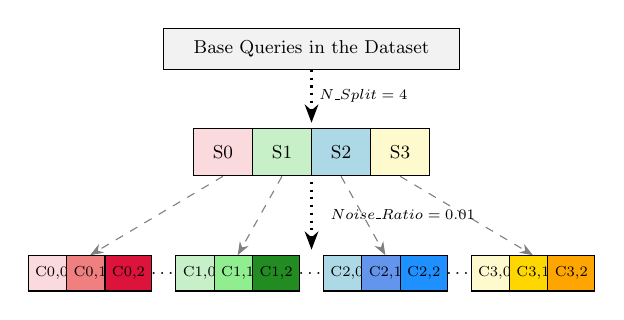
\begin{tikzpicture}[scale=0.75, transform shape, >=Stealth, font=\small]
    % Define local colors
    \definecolor{c0l}{RGB}{250, 218, 221} \definecolor{c0m}{RGB}{240, 128, 128} \definecolor{c0d}{RGB}{220, 20, 60}
    \definecolor{c1l}{RGB}{200, 240, 200} \definecolor{c1m}{RGB}{144, 238, 144} \definecolor{c1d}{RGB}{34, 139, 34}
    \definecolor{c2l}{RGB}{173, 216, 230} \definecolor{c2m}{RGB}{100, 149, 237} \definecolor{c2d}{RGB}{30, 144, 255}
    \definecolor{c3l}{RGB}{255, 250, 205} \definecolor{c3m}{RGB}{255, 215, 0}   \definecolor{c3d}{RGB}{255, 165, 0}

    % LEVEL 1: Base Queries
    \node[draw, fill=gray!10, minimum width=5cm, minimum height=0.7cm] (base) at (0, 0) {Base Queries in the Dataset};
    
    % LEVEL 2: Split Nodes (S0 - S3)
    \foreach \i/\col in {0/c0l, 1/c1l, 2/c2l, 3/c3l} {
        \node[draw, fill=\col, minimum width=1.0cm, minimum height=0.8cm] (s\i) at ({(\i-1.5)*1.0}, -1.75) {S\i};
    }
    
    % LEVEL 3: Perturbations (C_i,j)
    \def\groupspace{2.5} % horizontal space between groups
    \foreach \i/\cbase in {0/c0, 1/c1, 2/c2, 3/c3} {
        \foreach \j in {0,1,2} {
            \pgfmathsetmacro{\xpos}{(\i-1.5)*\groupspace + (\j-1)*0.65}
            \ifcase\j \colorlet{cc}{\cbase l} \or \colorlet{cc}{\cbase m} \or \colorlet{cc}{\cbase d} \fi
            \node[draw, fill=cc, minimum size=0.6cm] (c\i\j) at (\xpos, -3.8) {\scriptsize C\i,\j};
            
            % Dotted guides from S to middle child
            \ifnum\j=1
                \draw[->, gray, thin, dashed] (s\i.south) -- (c\i\j.north);
            \fi
        }
        
        % Dots between groups
        \ifnum\i>0
            \path (c\the\numexpr\i-1\relax2.east) -- (c\i0.west) node[midway] {\dots};
        \fi
    }

    % Main logic arrows
    \draw[->, dotted, thick] (base.south) -- (0, -1.25) node[midway, right] {\scriptsize $N\_Split=4$};
    
    % Middle label area
    \node[right] at (0.2, -2.8) {\scriptsize $Noise\_Ratio=0.01$};
    \draw[->, dotted, thick] (0,-2.25) -- (0,-3.4);

\end{tikzpicture}

        \caption{Synthesizing Queries with Semantic (Spatial) Locality}
        \label{fig:query-perturbation}
    \end{subfigure}
    \hfill
    \begin{subfigure}[t]{0.48\textwidth}
        \centering
        \resizebox{0.8\textwidth}{!}{
            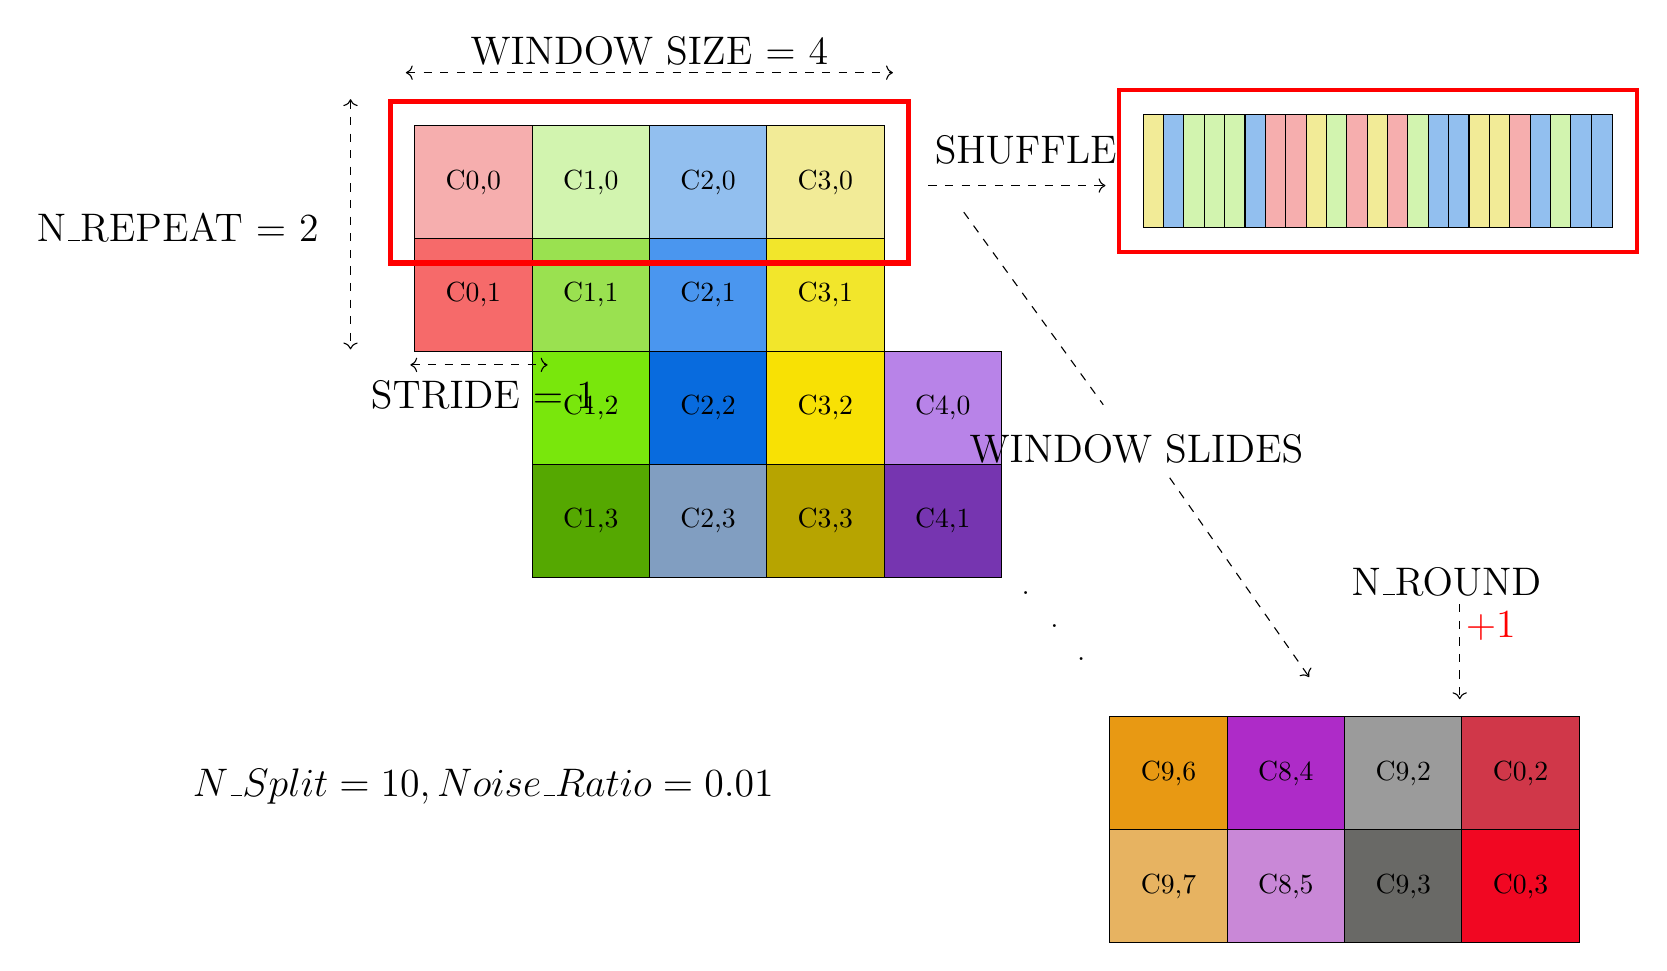
\begin{tikzpicture}[x=0.8pt,y=0.8pt,yscale=-1,xscale=1]

% --- CONFIGURATION ---
\def\cw{53} % Cell Width
\def\ch{51} % Cell Height
\definecolor{colorC0}{RGB}{246, 174, 174} % Light Red
\definecolor{colorC1}{RGB}{210, 244, 175} % Light Green
\definecolor{colorC2}{RGB}{146, 191, 239} % Light Blue
\definecolor{colorC3}{RGB}{242, 235, 151} % Light Yellow

% --- LEFT GRID (Main Grid) ---
% Row 0
\draw[fill=colorC0] (104, 64) rectangle ++(\cw,\ch) node[midway] {C0,0};
\draw[fill=colorC1] (157, 64) rectangle ++(\cw,\ch) node[midway] {C1,0};
\draw[fill=colorC2] (210, 64) rectangle ++(\cw,\ch) node[midway] {C2,0};
\draw[fill=colorC3] (263, 64) rectangle ++(\cw,\ch) node[midway] {C3,0};

% Row 1
\draw[fill={rgb,255:red,246; green,106; blue,106}] (104, 115) rectangle ++(\cw,\ch) node[midway] {C0,1};
\draw[fill={rgb,255:red,154; green,225; blue,80}]  (157, 115) rectangle ++(\cw,\ch) node[midway] {C1,1};
\draw[fill={rgb,255:red,74;  green,150; blue,239}] (210, 115) rectangle ++(\cw,\ch) node[midway] {C2,1};
\draw[fill={rgb,255:red,242; green,230; blue,43}]  (263, 115) rectangle ++(\cw,\ch) node[midway] {C3,1};

% Lower Blocks (Maintained colors from your original)
\draw[fill={rgb,255:red,121; green,231; blue,12}]  (157, 166) rectangle ++(\cw,\ch) node[midway] {C1,2};
\draw[fill={rgb,255:red,85;  green,168; blue,1}]   (157, 217) rectangle ++(\cw,\ch) node[midway] {C1,3};
\draw[fill={rgb,255:red,8;   green,107; blue,222}] (210, 166) rectangle ++(\cw,\ch) node[midway] {C2,2};
\draw[fill={rgb,255:red,129; green,158; blue,193}] (210, 217) rectangle ++(\cw,\ch) node[midway] {C2,3};
\draw[fill={rgb,255:red,248; green,225; blue,4}]   (263, 166) rectangle ++(\cw,\ch) node[midway] {C3,2};
\draw[fill={rgb,255:red,183; green,164; blue,0}]   (263, 217) rectangle ++(\cw,\ch) node[midway] {C3,3};
\draw[fill={rgb,255:red,184; green,131; blue,232}] (316, 166) rectangle ++(\cw,\ch) node[midway] {C4,0};
\draw[fill={rgb,255:red,118; green,53;  blue,176}] (316, 217) rectangle ++(\cw,\ch) node[midway] {C4,1};

% --- RED FOCUS BOX (Left) ---
\draw [red, line width=2pt] (93, 53) rectangle (327, 126);

% --- SHUFFLE BOX (Top Right) ---
% Now filled completely using colors from the Window (C0, C1, C2, C3)
\foreach \i/\shufcol in {
    0/colorC3, 1/colorC2, 2/colorC1, 3/colorC1, 4/colorC1, 5/colorC2, 
    6/colorC0, 7/colorC0, 8/colorC3, 9/colorC1, 10/colorC0, 11/colorC3, 
    12/colorC0, 13/colorC1, 14/colorC2, 15/colorC2, 16/colorC3, 17/colorC3, 
    18/colorC0, 19/colorC2, 20/colorC1, 21/colorC2, 22/colorC2} 
{
    \draw[fill=\shufcol, draw=black, line width=0.4pt]
        (433 + \i*9.2, 59) rectangle ++(9.5, 51);
}
% Outline for the shuffle bar
\draw [red, line width=1.5pt] (422, 48) rectangle (656, 121);

% --- BOTTOM RIGHT GRID ---
\draw[fill={rgb,255:red,232; green,153; blue,19}] (418, 331) rectangle ++(\cw,\ch) node[midway] {C9,6};
\draw[fill={rgb,255:red,231; green,179; blue,97}] (418, 382) rectangle ++(\cw,\ch) node[midway] {C9,7};
\draw[fill={rgb,255:red,174; green,43;  blue,200}] (471, 331) rectangle ++(\cw,\ch) node[midway] {C8,4};
\draw[fill={rgb,255:red,201; green,136; blue,215}] (471, 382) rectangle ++(\cw,\ch) node[midway] {C8,5};
\draw[fill={rgb,255:red,155; green,155; blue,155}] (524, 331) rectangle ++(\cw,\ch) node[midway] {C9,2};
\draw[fill={rgb,255:red,105; green,105; blue,102}] (524, 382) rectangle ++(\cw,\ch) node[midway] {C9,3};
\draw[fill={rgb,255:red,208; green,55;  blue,73}]  (577, 331) rectangle ++(\cw,\ch) node[midway] {C0,2};
\draw[fill={rgb,255:red,241; green,7;   blue,34}]  (577, 382) rectangle ++(\cw,\ch) node[midway] {C0,3};

% --- TEXT AND ARROWS ---
\node at (210, 30) {\Large WINDOW SIZE = 4};
\draw [dashed, <->] (100, 40) -- (320, 40);

\node [anchor=east] at (65, 110) {\Large N\_REPEAT = 2};
\draw [dashed, <->] (75, 52) -- (75, 165);

\node [anchor=north] at (135, 175) {\Large STRIDE = 1};
\draw [dashed, <->] (102, 172) -- (164, 172);

\node [anchor=north] at (135, 350) {\Large $N\_Split=10, Noise\_Ratio = 0.01$};



\node at (380, 75) {\Large SHUFFLE};
\draw [dashed, ->] (336, 91) -- (416, 91);

\node at (430, 210) {\Large WINDOW SLIDES};
\draw [dashed, -] (352, 103) -- (415, 190);
\draw [dashed, ->] (445, 223) -- (508, 313);

\node at (570, 270) {\Large N\_ROUND};
\node [red] at (590, 290) {\Large +1};
\draw [dashed, ->] (576, 280) -- (576, 323);

\node at (380, 275) {.}; \node at (393, 290) {.}; \node at (405, 305) {.};

\end{tikzpicture}
        }
        \caption{Workload Generation with temporal-semantic Locality}
        \label{fig:sliding-window}
    \end{subfigure}
    \caption{Evaluation framework proposed in this paper for benchmarking vector caches, used to evaluate QVCache.}
    \label{fig:evaluation-framework}
\end{figure*}
\begin{figure*}[t]
    \centering
    \begin{subfigure}[t]{0.48\textwidth}
        \centering
        \includegraphics[width=\linewidth,trim=0 120 0 0,clip]{figures/perturbation.pdf}
        \caption{Synthesizing queries with semantic (spatial) locality.}
        \label{fig:query-perturbation}
    \end{subfigure}
    \hfill
    \begin{subfigure}[t]{0.48\textwidth}
        \centering
        \includegraphics[width=\linewidth,trim=0 120 0 0,clip]{figures/workload-generation.pdf}
        \caption{Workload generation with temporal–semantic locality.}
        \label{fig:sliding-window}
    \end{subfigure}
    \caption{Evaluation framework proposed in this paper for benchmarking vector caches, used to evaluate QVCache.}
    \label{fig:evaluation-framework}
    \vspace{-\baselineskip}
\end{figure*}

\section{Evaluation Framework}
%Real-world vector search workloads exhibit skewed access patterns \cite{298625SmartANN, incrementalivfindexmaintenance}, with spatially close queries recurring (i.e., {temporal-semantic locality}), but existing systems are typically evaluated without accounting for this behavior, which is inadequate for assessing vector caches. Standard benchmarks execute each query only once and report aggregate metrics such as average recall and latency, which is sufficient for evaluating standalone ANN systems but insufficient for understanding the cache behavior. 

Real-world vector search workloads exhibit skewed access patterns~\cite{298625SmartANN, incrementalivfindexmaintenance}, with spatially close queries recurring (i.e. \textit{temporal–semantic locality}). However, existing systems are typically evaluated without accounting for this behavior, which is inadequate for assessing vector caches. In standard benchmarks, queries provided in the datasets rarely have overlapping neighbors, and each query is executed only once; benchmarks then report aggregate metrics such as average recall and latency. While this is sufficient for evaluating standalone ANN systems, it is insufficient for understanding cache behavior due to the lack of temporal–semantic locality.

To address this, we propose a workload generation framework that produces query patterns exhibiting temporal-semantic locality at varying degrees. As illustrated in Figure \ref{fig:query-perturbation}, we first partition the queries from the dataset into $N_{\text{split}}$ disjoint subsets to model shifts in the working set of the workload. 
Within each subset (split), we generate perturbed variants for each query to model the temporal-semantic locality. For a query $q$, we sample a random vector $r$ from the data vectors in the dataset and produce  

\begin{equation}
q' = (1-\eta) \cdot q + \eta \cdot r
\label{exp:perturbation-expression}
\end{equation}

\noindent where $\eta$ controls the noise ratio. This interpolation yields queries that are semantically similar, i.e., spatially close, while remaining distinct. % enabling evaluation of vector caches. 
As shown in Figure \ref{fig:overlap-analysis}, the similarity between the base and perturbed queries' neighbor sets decreases sharply with increased noise. At $\eta = 0.01$, roughly 95\% of nearest neighbors overlap, simulating queries that differ in phrasing but share similar intent.


As visualized in Figure \ref{fig:sliding-window}, to generate recurrence of spatially close queries and drifts in the working set, we employ a windowed query pattern \cite{10.14778/2735461.2735465inmemoryperformanceforbigdata}. Each window consists of perturbed versions of $WINDOW\_SIZE$ many base splits. Queries within the window are randomly shuffled and dispatched to the system, repeating $N_{\text{repeat}}$ times. After each repetition, $stride$ out of $WINDOW\_SIZE$ perturbed splits are replaced with new ones. This process continues until the window reaches the last splits, and the cycle can optionally be repeated $N_{\text{round}}$ times with fresh perturbed copies.

The parameter $WINDOW\_SIZE$ controls the working set size (i.e., the number of vectors brought into the cache per window) of the workload. $N_{\text{repeat}}$ measures short-term memory, i.e., the ability to capture cache hits within a short time window, while $N_{\text{round}}$ measures long-term memory across multiple cycles. The ratio $stride/WINDOW\_SIZE$ adjusts how quickly the working set drifts \label{sec:drift-amount} \cite{10.14778/2735461.2735465inmemoryperformanceforbigdata}. Together, these parameters allow us to generate workloads with varying locality and temporal characteristics, enabling comprehensive evaluation of vector caches.

\begin{table}[!htbp]
\centering
\small
\begin{tabular}{lrrrr}
\toprule
\textbf{Dataset} & \textbf{\#Vectors} & \textbf{Dim.} & \textbf{Distance} & \textbf{\#Queries} \\
\midrule
SIFT        & 1{,}000{,}000{,}000 & 128 & L2     & 10{,}000 \\
SpaceV\footnotemark[1] & 100{,}000{,}000     & 100 & L2     & 29{,}316 \\
DEEP\footnotemark[1]   & 10{,}000{,}000      & 96  & L2     & 10{,}000 \\
GIST        & 1{,}000{,}000       & 960 & L2     & 1{,}000 \\
GloVe       & 1{,}000{,}000       & 100 & Cosine & 10{,}000 \\
\bottomrule
\end{tabular}
\caption{Dataset statistics}
\label{tab:datasets}
\end{table}

\footnotetext[1]{For \textsc{SpaceV} and \textsc{DEEP}, we use the first 100M and 10M vectors of the 1B vectors in respective datasets.}

\section{Experiments}

\subsection{Experimental Setup}
We implement QVCache in C++, together with Python bindings. All experiments are conducted on a Linux system in a containerized Docker environment, equipped with an Intel Xeon Gold 5118 processor, 2.30GHz, with 24 physical cores, 376GB of DDR4 RAM, and a Dell Express Flash PM1725a 1.6TB NVMe SSD.

\textbf{Datasets.} We evaluate how well QVCache generalizes across diverse data by benchmarking it on five datasets that differ in scale, domain, and dimensionality, as summarized in Table~\ref{tab:datasets} \cite{sift, deep, gist, pennington-etal-2014-glove, SPACEV1B_SPTAG}. 

\textbf{Backends.} We evaluate QVCache across a range of backend databases to understand its performance under diverse scenarios. We employ the DiskANN \cite{diskann} implementation by Yu et al. (2025) \cite{yu2025topologyawarelocalizedupdatestrategy}, a state-of-the-art disk-based vector search framework, for benchmarking QVCache across multiple datasets. Additionally, we test QVCache with FAISS \cite{faiss}, pgvector \cite{pgvector}, Qdrant \cite{qdrant2025}, Pinecone \cite{pinecone}, and SPANN \cite{spann} to assess its effectiveness with backends that differ in storage model (in-memory, disk-based, or hybrid), deployment model (on-premises vs. cloud-based), and index type (graph, tree, etc.).

\textbf{Metrics.} %We evaluate QVCache using six metrics, as illustrated in Figures \ref{fig:dataset-experiments} and \ref{fig:backend-experiments}. Metrics are collected at the granularity of window steps, with each dot representing a step. 
We evaluate QVCache across six metrics measured per window, with values reported at window-step granularity, where each point in the figures corresponds to a single step.
\emph{Cache hit ratio} measures the fraction of queries served by QVCache without forwarding requests to the backend database, while \emph{Hit latency} captures the latency of these queries. We use P50 latency and omit P99 latency because, unless QVCache achieves a hit ratio above 99\%, P99 is dominated by queries that miss the cache and are served by the backend, yielding no meaningful distinction when using QVCache. %Instead, we use P50 latency to evaluate overall latency performance. %, independent of cache hits or misses.
Although QVCache is primarily designed for low-latency responses, it also improves throughput; we report the metric reflecting this benefit. To measure query accuracy, we use 10-recall@10. We also track the number of vectors retrieved from the backend into the cache over time to assess eviction behavior. 

\begin{figure*}[t]
\centering
% Define the column width for 5 columns (Using 0.195\textwidth for slight height increase)
\newlength{\colwidth}
\setlength{\colwidth}{0.195\textwidth}

% Column Order: sift, spacev100m, deep10m, text2image, glove

% ===== Row 1: hit_ratio =====
\begin{subfigure}{\colwidth}
    \includegraphics[width=\linewidth]{plots/dataset_experiments/bigann/hit_ratio.pdf}
\end{subfigure}
\begin{subfigure}{\colwidth}
    \includegraphics[width=\linewidth]{plots/dataset_experiments/spacev1b_100m/hit_ratio.pdf}
\end{subfigure}
\begin{subfigure}{\colwidth}
    \includegraphics[width=\linewidth]{plots/dataset_experiments/deep10m/hit_ratio.pdf}
\end{subfigure}
\begin{subfigure}{\colwidth}
    \includegraphics[width=\linewidth]{plots/dataset_experiments/gist/hit_ratio.pdf}
\end{subfigure}
\begin{subfigure}{\colwidth}
    \includegraphics[width=\linewidth]{plots/dataset_experiments/glove/hit_ratio.pdf}
\end{subfigure}
\\ % Add vertical space between rows

% ===== Row 2: avg_hit_latency (where the "shift" was observed) =====
\begin{subfigure}{\colwidth}
    \includegraphics[width=\linewidth]{plots/dataset_experiments/bigann/avg_hit_latency.pdf}
\end{subfigure}
\begin{subfigure}{\colwidth}
    \includegraphics[width=\linewidth]{plots/dataset_experiments/spacev1b_100m/avg_hit_latency.pdf}
\end{subfigure}
\begin{subfigure}{\colwidth}
    \includegraphics[width=\linewidth]{plots/dataset_experiments/deep10m/avg_hit_latency.pdf}
\end{subfigure}
\begin{subfigure}{\colwidth}
    \includegraphics[width=\linewidth]{plots/dataset_experiments/gist/avg_hit_latency.pdf}
\end{subfigure}
\begin{subfigure}{\colwidth}
    \includegraphics[width=\linewidth]{plots/dataset_experiments/glove/avg_hit_latency.pdf}
\end{subfigure}
\\ % Add vertical space between rows

% ===== Row 3: p50_latency =====
\begin{subfigure}{\colwidth}
    \includegraphics[width=\linewidth]{plots/dataset_experiments/bigann/p50_latency.pdf}
\end{subfigure}
\begin{subfigure}{\colwidth}
    \includegraphics[width=\linewidth]{plots/dataset_experiments/spacev1b_100m/p50_latency.pdf}
\end{subfigure}
\begin{subfigure}{\colwidth}
    \includegraphics[width=\linewidth]{plots/dataset_experiments/deep10m/p50_latency.pdf}
\end{subfigure}
\begin{subfigure}{\colwidth}
    \includegraphics[width=\linewidth]{plots/dataset_experiments/gist/p50_latency.pdf}
\end{subfigure}
\begin{subfigure}{\colwidth}
    \includegraphics[width=\linewidth]{plots/dataset_experiments/glove/p50_latency.pdf}
\end{subfigure}
\\ % Add vertical space between rows

% ===== Row 4: qps =====
\begin{subfigure}{\colwidth}
    \includegraphics[width=\linewidth]{plots/dataset_experiments/bigann/qps.pdf}
\end{subfigure}
\begin{subfigure}{\colwidth}
    \includegraphics[width=\linewidth]{plots/dataset_experiments/spacev1b_100m/qps.pdf}
\end{subfigure}
\begin{subfigure}{\colwidth}
    \includegraphics[width=\linewidth]{plots/dataset_experiments/deep10m/qps.pdf}
\end{subfigure}
\begin{subfigure}{\colwidth}
    \includegraphics[width=\linewidth]{plots/dataset_experiments/gist/qps.pdf}
\end{subfigure}
\begin{subfigure}{\colwidth}
    \includegraphics[width=\linewidth]{plots/dataset_experiments/glove/qps.pdf}
\end{subfigure}
\\ % Add vertical space between rows

% ===== Row 5: recall =====
\begin{subfigure}{\colwidth}
    \includegraphics[width=\linewidth]{plots/dataset_experiments/bigann/recall.pdf}
\end{subfigure}
\begin{subfigure}{\colwidth}
    \includegraphics[width=\linewidth]{plots/dataset_experiments/spacev1b_100m/recall.pdf}
\end{subfigure}
\begin{subfigure}{\colwidth}
    \includegraphics[width=\linewidth]{plots/dataset_experiments/deep10m/recall.pdf}
\end{subfigure}
\begin{subfigure}{\colwidth}
    \includegraphics[width=\linewidth]{plots/dataset_experiments/gist/recall.pdf}
\end{subfigure}
\begin{subfigure}{\colwidth}
    \includegraphics[width=\linewidth]{plots/dataset_experiments/glove/recall.pdf}
\end{subfigure}

% ===== Row 6: Memory Active Vectors =====
\begin{subfigure}{\colwidth}
    \includegraphics[width=\linewidth]{plots/dataset_experiments/bigann/memory_active_vectors.pdf}
\end{subfigure}
\begin{subfigure}{\colwidth}
    \includegraphics[width=\linewidth]{plots/dataset_experiments/spacev1b_100m/memory_active_vectors.pdf}
\end{subfigure}
\begin{subfigure}{\colwidth}
    \includegraphics[width=\linewidth]{plots/dataset_experiments/deep10m/memory_active_vectors.pdf}
\end{subfigure}
\begin{subfigure}{\colwidth}
    \includegraphics[width=\linewidth]{plots/dataset_experiments/gist/memory_active_vectors.pdf}
\end{subfigure}
\begin{subfigure}{\colwidth}
    \includegraphics[width=\linewidth]{plots/dataset_experiments/glove/memory_active_vectors.pdf}
\end{subfigure}

% ===== Row 7: Column captions (Datasets) =====
\begin{subfigure}{\colwidth}
    \centering
    \vspace{0.8em}
    (a) \textbf{SIFT}
\end{subfigure}
\begin{subfigure}{\colwidth}
    \centering
    \vspace{0.8em}
    (b) \textbf{SpaceV}
\end{subfigure}
\begin{subfigure}{\colwidth}
    \centering
    \vspace{0.8em}
    (c) \textbf{DEEP}
\end{subfigure}
\begin{subfigure}{\colwidth}
    \centering
    \vspace{0.8em}
    (d) \textbf{GIST}
\end{subfigure}
\begin{subfigure}{\colwidth}
    \centering
    \vspace{0.8em}
    (e) \textbf{GloVe}
\end{subfigure}

\caption{Vector search performance of backend vector database (DiskANN) alone vs. backend augmented with QVCache on the five datasets. $k$ is set to 10.}

\label{fig:dataset-experiments}
\end{figure*}

\subsection{Adaptive Query-Aware Caching}
\label{sec:dataset-experiments}

A query-aware vector cache must adopt to non-stationary workloads, where the active working set drifts \cite{10.14778/2735461.2735465inmemoryperformanceforbigdata} over time. It should support varying dimensionalities, distance functions, and $k$ values while requiring minimal configuration (i.e., without manually tuning similarity thresholds), regardless of the underlying dataset.

%To evaluate these properties, we conduct experiments on five datasets, as shown in 
Figures \ref{fig:dataset-experiments} and \ref{fig:k-experiments} show the results. Workloads are generated with $N_{\text{split}} = 10$, $\eta = 0.01$, $N_{\text{repeat}} = 3$, and $stride = 1$. QVCache is configured with $\alpha = 0.9$, $n_{\text{buckets}} = 8$, $d_{\text{reduced}} = 16$, and $n_{\text{mini-index}} = 4$. The value of $D$ is set to 0.25 for SIFT, 0.001 for GloVe, and 0.075 for the remaining datasets. \texttt{ADAPTIVE} search strategy is used to scan mini-indexes.  The capacity of each mini-index, $c_{\text{mini-index}}$, is set per dataset to approximate the working set size, defined as the number of unique vectors appearing in query neighbor sets within a window. Hence, this determines the number of vectors to be retrieved by QVCache. 

Queries are processed by $t_{processing} = 24$ worker threads, while asynchronous tasks, including vector insertions and threshold learning, are handled by a separate pool of $t_{processing} = 16$ threads.

As shown in Figure~\ref{fig:dataset-experiments}, the hit ratios for datasets such as SpaceV and GIST stabilize around 0.75, while the remaining datasets reach a hit ratio of 1, representing ideal behavior, during the second and third window repetitions. Each decline in hit ratio corresponds to a window slide. Throughput and median p50 latency closely follow the hit ratio, with QVCache configurations achieving up to 50x higher throughput. Integrating QVCache with DiskANN reduces p50 latency by 40x to 300x compared to the DiskANN-only configuration.

Recall is minimally affected. SIFT, SpaceV, and DEEP show approximately 2\% drops, while GIST and GloVe reach 6–12\% at some points. This trade-off between hit ratio and recall can be tuned using the deviation factor $D$, as discussed in Section 6.5.

Cache hits achieve sub-millisecond latency on SIFT, SpaceV, and DEEP, approximately 0.2 to 0.4 milliseconds, with slightly higher latencies on other datasets, approximately 0.6 to 1.0 milliseconds. For GIST, the higher latency results from its 960-dimensional vectors, which increase computational cost. In GloVe, despite comparable mini-index capacity, hit latency is higher due to the sequential scanning strategy across all mini-indexes.

Finally, as shown in Figure \ref{fig:k-experiments}, QVCache adapts to queries with varying $k$ values without any additional configuration beyond the total cache capacity. Capacities of 6,000, 60,000, and 600,000 vectors were allocated for $k = 1$, 10, and 100, respectively, reflecting the linear increase in vectors retrieved per window as $k$ grows. Overall, performance trends remain consistent across different $k$ values, with latency improvements becoming more pronounced for larger $k$.


\begin{figure}[h]
    \centering

    % Top row
    \begin{subfigure}[t]{0.48\linewidth}
        \centering
        \includegraphics[width=\linewidth]{plots/k_experiments/all_comparison/hit_ratio.pdf}
    \end{subfigure}\hfill
    \begin{subfigure}[t]{0.48\linewidth}
        \centering
        \includegraphics[width=\linewidth]{plots/k_experiments/all_comparison/memory_active_vectors.pdf}
    \end{subfigure}

    \vspace{0.75em}

    % Bottom row
    \begin{subfigure}[t]{0.48\linewidth}
        \centering
        \includegraphics[width=\linewidth]{plots/k_experiments/all_comparison/recall.pdf}
    \end{subfigure}
    \begin{subfigure}[t]{0.48\linewidth}
        \centering
        \includegraphics[width=\linewidth]{plots/k_experiments/all_comparison/p50_latency.pdf}
    \end{subfigure}

    \caption{Effect of varying $k$ on SIFT dataset.}
    \label{fig:k-experiments}
\end{figure}

\subsection{Sensitivity to Cache Capacity and Mini Index Partitioning}

As first noted by Belady \cite{belady1966study}, an ideal cache would retain exactly the items that will be accessed again and evict only those that will never be referenced in the future. Such optimal behavior is attainable only with an unbounded cache or an oracle that perfectly predicts future accesses. Since neither assumption is practical, real systems are inherently constrained by finite capacity and imperfect eviction decisions. The same limitations apply to QVCache.

To assess how well QVCache maintains high hit ratios under fixed capacity, we repeat the experiment from Figure \ref{fig:dataset-experiments} on the SIFT dataset using identical parameters, except with $N_{\text{round}} = 2$, as shown in Figure \ref{fig:cache_size_experiments}. Perturbed copies of a base split within a window bring approximately 15,000 vectors into the cache. With a window size of 4, the working set therefore contains roughly 60,000 vectors. Since the stride is 1, the working set changes by about 25\% at each window slide. An ideal configuration for this workload would thus set $c_{\text{mini-index}} = 15{,}000$ and a total cache capacity of at least 60,000 vectors.

In practice, however, estimating working set sizes and shift rates can be difficult. We therefore examine QVCache’s sensitivity to total cache capacity and $c_{\text{mini-index}}$ in Figure \ref{fig:cache_size_experiments}. On the left, we fix $c_{\text{mini-index}}$ at 15,000 and vary the total cache capacity. When the capacity is sufficient to hold the working set, the hit ratio remains high and ideally converges to 1. When capacity is insufficient, QVCache exhibits the expected degradation in hit ratio, similar to conventional caches, while recall remains largely unaffected.

On the right, we fix the total cache capacity at 60,000 and vary $c_{\text{mini-index}}$. We find that $c_{\text{mini-index}}$ has little impact on overall hit ratio and recall. However, larger mini-indexes result in more information being evicted at once. If recently evicted vectors are accessed again shortly afterward, this can temporarily reduce the hit ratio. Consequently, partitioning the total capacity across multiple mini-indexes is generally preferable, although this introduces additional hit latency, as discussed in Section 6.4.

\begin{figure}[h]
\centering

% Two columns → ~0.48 of column width each
\setlength{\colwidth}{0.48\columnwidth}

% ===== Row 1: hit_ratio =====
\begin{subfigure}{\colwidth}
    \includegraphics[width=\linewidth]{plots/total_cache_size_experiments/hit_ratio.pdf}
\end{subfigure}
\begin{subfigure}{\colwidth}
    \includegraphics[width=\linewidth]{plots/partitioning_experiments/hit_ratio.pdf}
\end{subfigure}
\\[0.5em]

% ===== Row 2: recall =====
\begin{subfigure}{\colwidth}
    \includegraphics[width=\linewidth]{plots/total_cache_size_experiments/recall.pdf}
\end{subfigure}
\begin{subfigure}{\colwidth}
    \includegraphics[width=\linewidth]{plots/partitioning_experiments/recall.pdf}
\end{subfigure}
\\[0.5em]

% ===== Row 3: memory_active_vectors =====
\begin{subfigure}{\colwidth}
    \includegraphics[width=\linewidth]{plots/total_cache_size_experiments/memory_active_vectors.pdf}
\end{subfigure}
\begin{subfigure}{\colwidth}
    \includegraphics[width=\linewidth]{plots/partitioning_experiments/memory_active_vectors.pdf}
\end{subfigure}
\\[0.8em]

% ===== Column Labels =====
\begin{subfigure}{\colwidth}
    \centering
    (a) Cache capacity
\end{subfigure}
\begin{subfigure}{\colwidth}
    \centering
    (b) Mini-index capacity
\end{subfigure}

\caption{
Effect of cache capacity and size of mini-indexes in QVCache on the SIFT dataset.
Left: varying total cache capacity via $n_{\text{mini-index}}$.
Right: varying $c_{\text{mini-index}}$ with fixed total capacity.}
\label{fig:cache_size_experiments}
\end{figure}


\begin{figure}[h]
    \centering

    \begin{subfigure}{0.7\linewidth}
        \centering
        \includegraphics[width=\linewidth]{plots/granularity_experiments/avg_hit_latency.pdf}
        \label{fig:plot1}
    \end{subfigure}

    \caption{Effect of mini-index granularity on QVCache performance. The total cache capacity is fixed at 50{,}000 vectors, while the number of mini-indexes is varied to control per–mini-index capacity.
}
    \label{fig:granularity-effect}
\end{figure}

\subsection{Granularity Matters: Balancing Eviction Cost and Hit Latency}

The granularity at which data is stored and retrieved has been extensively studied for decades. This includes classic work on page-size selection in database buffer pools and operating system caches~\cite{gray1998fiveminuteruleyearslater,7816668}, as well as more recent studies in cloud database systems, where access costs to remote storage layers are significantly higher~\cite{Zimmerer_2025}. These works explore different trade-offs, such as balancing I/O amortization against eviction cost and cache efficiency. For example, modern analytical systems like Snowflake~\cite{10.1145/2882903.2903741} store data in micropartitions to carefully balance parallelism, metadata overhead, and networked storage access costs. In traditional database systems, this problem is typically framed as finding an appropriate balance between the number of I/O operations required per record access and the effectiveness of the buffer cache.

Larger mini-indexes incur higher information loss upon eviction, as evicting a single mini-index removes a larger set of cached vectors at once. In the extreme case where $n_{\text{mini-index}} = 1$, the entire cache contents are evicted upon the first cache miss after the cache reaches full capacity. This motivates partitioning the cache into finer-grained units using multiple mini-indexes, thereby reducing eviction-induced information loss.

However, this increased granularity comes at a cost. Reducing the capacity of each mini-index can negatively impact cache-hit latency. The FreshVamana algorithm reduces the number of distance computations logarithmically with respect to the index size. Splitting a single FreshVamana index into multiple smaller mini-indexes diminishes this benefit. As a result, the cost of a cache-hit search can be approximated as
\[
C(N) \propto n_{\text{mini-index}} \cdot \log\!\left(\frac{N}{n_{\text{mini-index}}}\right),
\]
where $N$ denotes the total cache capacity in terms of vectors. Consequently, the cache cannot be arbitrarily partitioned into increasingly smaller mini-indexes, as the linear increase in the number of mini-indexes eventually outweighs the logarithmic reduction in per-index search cost.

To further analyze this trade-off, we conducted the experiment shown in Figure~\ref{fig:granularity-effect} using the SIFT dataset. We fixed the total cache capacity and varied the number of mini-indexes, $n_{\text{mini-index}}$, which implicitly determines the capacity of each mini-index, $c_{\text{mini-index}}$. All other parameters were kept identical to those described in Section~5.3. As $n_{\text{mini-index}}$ increases, the average cache-hit latency rises, since the scanning strategy must probe a larger number of mini-indexes before identifying a confident candidate neighbor set.

Based on our experimental results, QVCache capacity should not be scaled vertically by indefinitely increasing $c_{\text{mini-index}}$. Instead, horizontal scaling through the addition of multiple mini-indexes is preferable, as it reduces eviction-induced information loss. However, this partitioning should not be pushed beyond the point where an individual mini-index can no longer accommodate a working set, as overly fine-grained partitioning degrades cache-hit latency.


\begin{figure}[h]
    \centering
    \begin{subfigure}{0.48\linewidth}
        \centering
        \includegraphics[width=\linewidth]{plots/deviation_factor_experiments/hit_ratio.pdf}
    \end{subfigure}\hfill
    \begin{subfigure}{0.48\linewidth}
        \centering
        \includegraphics[width=\linewidth]{plots/deviation_factor_experiments/recall.pdf}
    \end{subfigure}

    \caption{Deviation Factor Effect on Hit Ratio - Recall on SIFT}
    \label{fig:deviation-factor-experiment}
\end{figure}

\subsection{Controlling Recall and Cache Hit Ratio via Deviation Factor}

QVCache dynamically adjusts similarity thresholds during execution. In addition, it allows explicit control over the trade-off between recall and cache hit ratio through the deviation factor, $D$.

We conducted an experiment on the SIFT dataset in which all settings were kept identical to those described in Section 6.2, except that $D$ was varied as a controlled parameter. The results, shown in Figure~\ref{fig:deviation-factor-experiment}, demonstrate that increasing $D$ leads to a higher cache hit ratio at the cost of reduced recall. In practice, this trade-off exhibits a saturation effect: beyond a certain point, further increasing $D$ yields diminishing improvements in hit ratio and only marginal reductions in recall.

There is no universal rule for selecting an appropriate deviation factor, as it depends on multiple factors including the dataset, vector dimensionality, query distribution, and distance metric. We therefore recommend initializing $D$ with a conservative value and gradually increasing it while monitoring recall and hit-ratio metrics. Since QVCache does not maintain any internal state that depends on $D$, adjusting this parameter can be performed online without requiring system downtime.


\begin{figure}[h]
    \centering

    \begin{subfigure}{0.7\linewidth}
        \centering
        \includegraphics[width=\linewidth]{plots/spatial_threshold_experiments/recall.pdf}
        \label{fig:plot1}
    \end{subfigure}

    \caption{Impact of Global vs. Spatial Threshold(s) on Recall}
    \label{fig:spatial-threshold-experiment}
\end{figure}


\subsection{Spatial Thresholds Are Key to Correct Cache Hit/Miss Decisions}
Vector distributions vary significantly across the vector space: some regions are densely clustered, while others are sparse. This heterogeneity makes it impractical to rely on a single global similarity threshold for all cache hit decisions.

To evaluate this effect, we repeated the experiment from Section 5.2 on the SIFT dataset under two configurations: one using a single global threshold and the other using spatial thresholds. As shown in Figure~\ref{fig:spatial-threshold-experiment}, the global threshold aggregates updates from cache misses across all regions, failing to capture local patterns and causing up to a 15\% loss in recall due to incorrect hit/miss decisions. In contrast, spatial thresholds adapt to local variations in the query distribution, limiting recall degradation to at most 2–3\%, demonstrating their effectiveness in preserving the backend database’s accuracy.


\begin{figure}[h]
    \centering

    % Row 1: Hit Ratio
    \begin{minipage}{0.48\linewidth}
        \centering
        \includegraphics[width=\linewidth]{plots/pca_experiments/d_reduced/hit_ratio.pdf}
        \subcaption{$d_{\text{reduced}}$ — Hit Ratio}
    \end{minipage}\hfill
    \begin{minipage}{0.48\linewidth}
        \centering
        \includegraphics[width=\linewidth]{plots/pca_experiments/n_buckets/hit_ratio.pdf}
        \subcaption{$n_{\text{buckets}}$ — Hit Ratio}
    \end{minipage}

    \vspace{0.8em}

    % Row 2: Recall
    \begin{minipage}{0.48\linewidth}
        \centering
        \includegraphics[width=\linewidth]{plots/pca_experiments/d_reduced/recall.pdf}
        \subcaption{$d_{\text{reduced}}$ — Recall}
    \end{minipage}\hfill
    \begin{minipage}{0.48\linewidth}
        \centering
        \includegraphics[width=\linewidth]{plots/pca_experiments/n_buckets/recall.pdf}
        \subcaption{$n_{\text{buckets}}$ — Recall}
    \end{minipage}

    \caption{Impact of granularity of space partitioning and dimensionality reduction on recall and hit ratio. Left: varying $d_{\text{reduced}}$ (fixed $n_{\text{buckets}}$ to 8). Right: varying $n_{\text{buckets}}$ (fixed $d_{\text{reduced}}$ to 16).}

    \label{fig:pca_experiments}
\end{figure}


\subsection{Sensitivity Analysis: Space Partitioning and Dimensionality Reduction}

We evaluate QVCache’s sensitivity to the granularity of space partitioning ($n_{buckets}$) and dimensionality reduction ($d_{reduced}$) by repeating the experiment from Figure \ref{fig:dataset-experiments} on the GIST dataset with $WINDOW\_SIZE = 1$ and $stride = 1$. As shown in Figure \ref{fig:pca_experiments}, the left column fixes $n_{buckets}$ at 8 and varies $d_{reduced}$, while the right column fixes $d_{reduced}$ at 16 and varies $n_{buckets}$, reporting the resulting hit ratio and recall.

GIST vectors have 960 dimensions. Increasing $d_{reduced}$ to 128 or higher provides only a modest improvement in recall (around 3–4\%) while significantly reducing the hit ratio, highlighting the effectiveness of dimensionality reduction for guiding cache hit–miss decisions.

Similarly, increasing $n_{buckets}$ from 8 to 128 yields an average recall improvement of roughly 5\% but heavily reduces the hit ratio. This behavior arises because Algorithm \ref{alg:learn-threshold} overfits local patterns (i.e. the partitioning is so fine-grained that $\theta[k][R]$ learns almost a query-specific estimate of $\text{d}{_\text{backend}}[k]$ in each region) and fails to generalize across queries.

\begin{table}[h]
\centering
\captionsetup{skip=6pt}
\small % Reduces font size; use \footnotesize for even smaller
\renewcommand{\arraystretch}{1.0} % Reduced from 1.15
\setlength{\tabcolsep}{4pt}    % Reduced from 6pt

\begin{tabular}{|>{\centering\arraybackslash}m{2.2cm}|c|c|c|c|c|c|}
\hline
\diagbox[width=2.2cm,height=0.9cm]
{$c_{\text{mini-index}}$}{$n_{\text{mini-index}}$}
& 1 & 2 & 4 & 8 & 16 & 32 \\
\hline
3{,}125
& \cellcolor{gray!25}16
& \cellcolor{orange!25}24
& \cellcolor{yellow!25}37
& \cellcolor{green!25}62
& \cellcolor{blue!25}113
& \cellcolor{purple!25}219 \\
\hline
6{,}250
& \cellcolor{orange!25}18
& \cellcolor{yellow!25}34
& \cellcolor{green!25}56
& \cellcolor{blue!25}100
& \cellcolor{purple!25}189
& \\
\hline
12{,}500
& \cellcolor{yellow!25}23
& \cellcolor{green!25}58
& \cellcolor{blue!25}99
& \cellcolor{purple!25}183
& & \\
\hline
25{,}000
& \cellcolor{green!25}34
& \cellcolor{blue!25}108
& \cellcolor{purple!25}170
& & & \\
\hline
50{,}000
& \cellcolor{blue!25}56
& \cellcolor{purple!25}171
& & & & \\
\hline
100{,}000
& \cellcolor{purple!25}99
& & & & & \\
\hline
\end{tabular}

\caption{Memory usage (in MB) of QVCache with varying
$n_{\text{mini-index}}$ and $c_{\text{mini-index}}$ (in vectors) on SIFT.}
\label{tab:memory-footprint-experiment}
\end{table}

\subsection{Memory Overhead Analysis of QVCache}

QVCache maintains only the hottest vectors in its cache and evicts entries once the allocated capacity is reached, ensuring memory usage never exceeds the configured limit. To quantify this, we replicate the experiment from Section \ref{sec:dataset-experiments} under varying cache capacities by adjusting $n_{mini-index}$ and $c_{mini-index}$, as summarized in Table \ref{tab:memory-footprint-experiment}.

For a billion-scale dataset such as SIFT, DiskANN requires 33.5 GB of memory. Adding QVCache with a capacity of 100,000 vectors incurs only 100–200 MB of overhead. Memory usage grows linearly with total capacity (and naturally with vector dimensionality), and partitioning across multiple mini-indexes further increases overhead, as shown by the diagonals in Table \ref{tab:memory-footprint-experiment}.


For workloads with working sets around 100,000 vectors, the overhead remains around 200 MB, suitable for client-side caching. When embedding QVCache directly into backend systems, extreme cases with working sets up to 1 million vectors result in roughly 2 GB of overhead. Considering that disk-based systems require tens of gigabytes and in-memory systems require hundreds of gigabytes, this overhead is negligible compared to the latency and throughput improvements enabled by QVCache.

Moreover, the memory required to store distance thresholds is negligible and is included in the numbers reported in Table \ref{tab:memory-footprint-experiment}. For example, QVCache learns roughly 1.5K, 15K, and 50K thresholds for GIST, SIFT, and SpaceV in Figure \ref{fig:dataset-experiments}, consuming about 200 KB for SpaceV. Even under pessimistic assumptions where, e.g., one million thresholds are learned due to highly diverse queries or varying values of $k$, the footprint remains around 4 MB. Users may optionally cap the number of stored thresholds, evicting and relearning them if needed. Overall, threshold storage contributes insignificantly to QVCache’s memory use.

\begin{figure}[h]
    \centering

    % Top row
    \begin{subfigure}[t]{0.48\linewidth}
        \centering
        \includegraphics[width=\linewidth]{plots/noise_ratio_experiments/hit_ratio.pdf}
    \end{subfigure}\hfill
    \begin{subfigure}[t]{0.48\linewidth}
        \centering
        \includegraphics[width=\linewidth]{plots/noise_ratio_experiments/recall.pdf}
    \end{subfigure}

    \vspace{0.75em}

    % Bottom row
    \begin{subfigure}[t]{0.48\linewidth}
        \centering
        \includegraphics[width=\linewidth]{plots/noise_ratio_experiments/p50_latency.pdf}
    \end{subfigure}
    \begin{subfigure}[t]{0.48\linewidth}
        \centering
        \includegraphics[width=\linewidth]{plots/noise_ratio_experiments/memory_active_vectors.pdf}
    \end{subfigure}

    \caption{Effect of increasing noise ratio, $\eta$, on DEEP dataset.}
    \label{fig:noise-ratio-experiments}
\end{figure}

\subsection{Stress-Testing QVCache in the Absence of Temporal–Semantic Locality}

In Figure~\ref{fig:noise-ratio-experiments}, we evaluate how the noise ratio $\eta$ affects QVCache by repeating the experiment from Section~\ref{sec:dataset-experiments} while increasing $\eta$ up to~0.6. To avoid triggering evictions and simply observe how many vectors QVCache retrieves into the cache, we set the cache capacity to 1M vectors. As shown in Figure~\ref{fig:overlap-analysis}, $\eta = 0.6$ represents the extreme case in which perturbed queries share no overlap in their top-$k$ neighbors, i.e., every query effectively becomes unique. Even under this setting, QVCache sustains high hit ratios while degrading recall by less than~4\%.

This result reveals an important phenomenon: pairwise uniqueness among queries does not imply global dissimilarity across a workload. Although no two perturbed queries share top-$k$ neighbors, the collective set of vectors they reference still exhibits overlap at scale. This is reflected in the curves for $\eta = 0.4$ and $\eta = 0.6$, where the number of vectors inserted into the cache increases only modestly. Thus, QVCache may remain effective even when similar queries do not repeat, leveraging potential collaboration across many unique queries rather than relying solely on strict temporal-semantic locality.





\begin{figure*}[t]
\centering

% Adjusted column width for 5 columns (roughly 1/5 of text width)
\setlength{\colwidth}{0.18\textwidth}

% ===== Row 1: hit_ratio =====
%\begin{subfigure}{\colwidth}
%    \includegraphics[width=\linewidth]{plots/backend_experiments/faiss/hit_ratio.pdf}
%\end{subfigure}
%\begin{subfigure}{\colwidth}
%    \includegraphics[width=\linewidth]{plots/backend_experiments/qdrant/hit_ratio.pdf}
%\end{subfigure}
%\begin{subfigure}{\colwidth}
%    \includegraphics[width=\linewidth]{plots/backend_experiments/pgvector/hit_ratio.pdf}
%\end{subfigure}
%\begin{subfigure}{\colwidth}
%    \includegraphics[width=\linewidth]{plots/backend_experiments/pinecone/hit_ratio.pdf}
%\end{subfigure}
%\begin{subfigure}{\colwidth}
%    \includegraphics[width=\linewidth]{plots/backend_experiments/sptag/hit_ratio.pdf}
%\end{subfigure}

% ===== Row 2: avg_hit_latency =====
%\begin{subfigure}{\colwidth}
%    \includegraphics[width=\linewidth]{plots/backend_experiments/faiss/avg_hit_latency.pdf}
%\end{subfigure}
%\begin{subfigure}{\colwidth}
%    \includegraphics[width=\linewidth]{plots/backend_experiments/qdrant/avg_hit_latency.pdf}
%\end{subfigure}
%\begin{subfigure}{\colwidth}
%    \includegraphics[width=\linewidth]{plots/backend_experiments/pgvector/avg_hit_latency.pdf}
%\end{subfigure}
%\begin{subfigure}{\colwidth}
%    \includegraphics[width=\linewidth]{plots/backend_experiments/pinecone/avg_hit_latency.pdf}
%\end{subfigure}
%\begin{subfigure}{\colwidth}
%    \includegraphics[width=\linewidth]{plots/backend_experiments/sptag/avg_hit_latency.pdf}
%\end{subfigure}

% ===== Row 3: p50_latency =====
\begin{subfigure}{\colwidth}
    \includegraphics[width=\linewidth]{plots/backend_experiments/faiss/p50_latency.pdf}
\end{subfigure}
\begin{subfigure}{\colwidth}
    \includegraphics[width=\linewidth]{plots/backend_experiments/qdrant/p50_latency.pdf}
\end{subfigure}
\begin{subfigure}{\colwidth}
    \includegraphics[width=\linewidth]{plots/backend_experiments/pgvector/p50_latency.pdf}
\end{subfigure}
\begin{subfigure}{\colwidth}
    \includegraphics[width=\linewidth]{plots/backend_experiments/pinecone/p50_latency.pdf}
\end{subfigure}
\begin{subfigure}{\colwidth}
    \includegraphics[width=\linewidth]{plots/backend_experiments/sptag/p50_latency.pdf}
\end{subfigure}

% ===== Row 4: qps =====
%\begin{subfigure}{\colwidth}
%    \includegraphics[width=\linewidth]{plots/backend_experiments/faiss/qps.pdf}
%\end{subfigure}
%\begin{subfigure}{\colwidth}
%    \includegraphics[width=\linewidth]{plots/backend_experiments/qdrant/qps.pdf}
%\end{subfigure}
%\begin{subfigure}{\colwidth}
%    \includegraphics[width=\linewidth]{plots/backend_experiments/pgvector/qps.pdf}
%\end{subfigure}
%\begin{subfigure}{\colwidth}
%    \includegraphics[width=\linewidth]{plots/backend_experiments/pinecone/qps.pdf}
%\end{subfigure}
%\begin{subfigure}{\colwidth}
%    \includegraphics[width=\linewidth]{plots/backend_experiments/sptag/qps.pdf}
%\end{subfigure}

% ===== Row 5: recall =====
\begin{subfigure}{\colwidth}
    \includegraphics[width=\linewidth]{plots/backend_experiments/faiss/recall.pdf}
\end{subfigure}
\begin{subfigure}{\colwidth}
    \includegraphics[width=\linewidth]{plots/backend_experiments/qdrant/recall.pdf}
\end{subfigure}
\begin{subfigure}{\colwidth}
    \includegraphics[width=\linewidth]{plots/backend_experiments/pgvector/recall.pdf}
\end{subfigure}
\begin{subfigure}{\colwidth}
    \includegraphics[width=\linewidth]{plots/backend_experiments/pinecone/recall.pdf}
\end{subfigure}
\begin{subfigure}{\colwidth}
    \includegraphics[width=\linewidth]{plots/backend_experiments/sptag/recall.pdf}
\end{subfigure}

% ===== Row 6: memory_active_vectors =====
%\begin{subfigure}{\colwidth}
%    \includegraphics[width=\linewidth]{plots/backend_experiments/faiss/memory_active_vectors.pdf}
%\end{subfigure}
%\begin{subfigure}{\colwidth}
%    \includegraphics[width=\linewidth]{plots/backend_experiments/qdrant/memory_active_vectors.pdf}
%\end{subfigure}
%\begin{subfigure}{\colwidth}
%    \includegraphics[width=\linewidth]{plots/backend_experiments/pgvector/memory_active_vectors.pdf}
%\end{subfigure}
%\begin{subfigure}{\colwidth}
%    \includegraphics[width=\linewidth]{plots/backend_experiments/pinecone/memory_active_vectors.pdf}
%\end{subfigure}
%\begin{subfigure}{\colwidth}
%    \includegraphics[width=\linewidth]{plots/backend_experiments/sptag/memory_active_vectors.pdf}
%\end{subfigure}

% ===== Row 7: Column captions =====
\begin{subfigure}{\colwidth}
    \centering
    \vspace{0.5em}
    \hspace{2em}(a) \textbf{FAISS}
\end{subfigure}
\begin{subfigure}{\colwidth}
    \centering
    \vspace{0.5em}
    \hspace{2em}(b) \textbf{Qdrant}
\end{subfigure}
\begin{subfigure}{\colwidth}
    \centering
    \vspace{0.5em}
    \hspace{2em}(c) \textbf{pgvector}
\end{subfigure}
\begin{subfigure}{\colwidth}
    \centering
    \vspace{0.5em}
    \hspace{2em}(d) \textbf{Pinecone}
\end{subfigure}
\begin{subfigure}{\colwidth}
    \centering
    \vspace{0.5em}
    \hspace{2em}(e) \textbf{SPANN}
\end{subfigure}

\caption{Performance of Various Backend Databases With and Without QVCache on DEEP Dataset}
\label{fig:backend-experiments}
\end{figure*}

\subsection{Backend-Agnostic Caching}

QVCache is compatible with any vector search system, independent of the underlying index type, system scale, or deployment environment, requiring only the implementation of standard search and fetch interfaces. To illustrate this property, we conduct the experiments shown in Figure \ref{fig:backend-experiments}, using the same parameter settings as in Section 6.2 for the DEEP dataset. All backends are evaluated both with and without QVCache. FAISS, Qdrant, and pgvector are deployed on the Linux host described in Section 6.2, while Pinecone is evaluated using its managed cloud service.

Pinecone \cite{pinecone}, a cloud-managed vector search service, exhibits relatively high latencies ($\approx$ 100 ms) due to network round-trip overheads. As shown in Figure \ref{fig:backend-experiments}, integrating QVCache on the client side bypasses this network latency and reduces p50 latency by up to three orders of magnitude ($\approx$ 1000×). Although cache-miss fetches may incur additional time, we observe no degradation in recall or hit-rate convergence. %Beyond latency reduction, QVCache also lowers serving costs for services billed on a per-query basis by converting a large fraction of requests into local, non-billable cache hits.

For hybrid memory–disk backends, such as Qdrant \cite{qdrant2025} and SPANN \cite{spann}, and disk-only backends like pgvector \cite{pgvector}, QVCache provides substantial latency improvements by fronting their client libraries. Specifically, we observe up to $\approx$100×, $\approx$300×, and $\approx$500× reductions in p50 latency for Qdrant, SPANN, and pgvector, respectively. While our experiments use client-side integration, embedding QVCache directly within these systems would enable cross-client caching, exploiting a global view of incoming queries and allowing multiple clients’ requests to be served more efficiently through better aggregation.

Even for fully in-memory backends such as FAISS, QVCache achieves up to 40× latency reduction. Here, both the backend and QVCache maintain indexes and vectors in memory, yet cache hits are faster because QVCache constrains the search space, allowing best-first search to converge in fewer steps. Nonetheless, QVCache introduces an in-cache probe for every request; when backend latency is already low and cache hit rates are limited, this overhead can be non-negligible.

In summary, augmenting a state-of-the-art in-memory backend such as FAISS with QVCache results in approximately $40\times$ lower p50 latency. For disk-based vector search systems, augmenting them with QVCache yields $\approx 100$–$\approx 500\times$ reductions in p50 latency, and for cloud-hosted systems such as Pinecone, the benefit is magnified to nearly $1000\times$ by eliminating network latency on cache hits.






\section{Related Work}

\textbf{Vector Databases:} The growing demand for managing embedding data has led to the development of numerous vector database management systems in recent years \cite{pinecone, pgvector, ZillizServerless2025, milvus, qdrant2025, OpenSearch, 10.14778/3685800.3685806-gaussdb}. These systems incorporate a variety of optimizations tailored to vector data, including storage architectures, lock management, and query processing. Moreover, several studies have explored accelerating ANN search using specialized hardware, including GPUs~\cite{bang,scalablegraphindexingusinggpus} and FPGAs~\cite{vector-search-delayed-fpga}. Furthermore, as vector data is increasingly combined with relational data, recent research has focused on supporting fundamental relational operations such as joins and filtering within vector databases, which are known as similarity joins \cite{Chen_2025} and filtered vector search \cite{10.14778/3750601.3750700}.

%\textbf{Vector Search Indexes:} Vector databases employ a variety of index structures to optimize performance while maintaining high recall in Approximate Nearest Neighbor (ANN) search. These structures include graph-based indexes \cite{diskann, HNSWMalkovY16, nsg, 9383170}, which organize vectors into navigable graphs for efficient neighbor exploration; tree-based indexes \cite{10.14778/3204028.3204034}, particularly effective for low-dimensional data; hash-based approaches \cite{locality-sensitive-hashing, jafari2021surveylocalitysensitivehashing}, which leverage hash functions to map similar vectors to the same buckets; and inverted indexes \cite{product-quantization, Lempitsky2015TheIM}, which partition the vector space into clusters and use quantization techniques to accelerate search while reducing memory usage.

%Initially, vector search was primarily performed over static collections, where the entire dataset was known in advance and the index could be built once. However, modern applications such as recommendation systems, online advertising, and real-time analytics require continuously evolving datasets. This has created a need for dynamic vector search indexes that can efficiently support the insertion of new vectors and the deletion of existing ones without rebuilding the entire index, since full rebuilds are computationally expensive and impractical for large-scale or streaming data. To address this, several dynamic indexing approaches have been developed \cite{mohoney2025quakeadaptiveindexingvector, xu2025inplaceupdatesgraphindex}, which aim to maintain high recall and query performance while performing updates incrementally. The main challenges they tackle include preserving the index structure quality, minimizing degradation of search accuracy, and ensuring efficient update operations in streaming or rapidly changing workloads.


\textbf{Caching in Vector Databases:}  Caching in vector databases typically refers to system-level mechanisms \cite{jeong2025callcontextawarelowlatencyretrieval, milvus, 10.14778/3685800.3685805, turbocharging-vector-databases-ssds, diskann, tiered-cache-hnsw} that are tightly coupled with their respective systems and underlying indexes. These approaches primarily aim to reduce the cost of disk accesses arising from random I/O during graph traversal. For example, \cite{diskann} caches nodes near traversal entry points in memory, \cite{tiered-cache-hnsw} keeps the uppermost HNSW layer resident in memory, \cite{jeong2025callcontextawarelowlatencyretrieval} batches queries by aligning their page requests, and \cite{turbocharging-vector-databases-ssds} reorganizes the on-disk index layout to minimize page-cache misses.


\textbf{Similarity Caching:}
Similarity based caching has recently gained traction in the context of Large Language Model (LLM) APIs and document retrieval. The core idea is to place a query level cache in front of the model or retrieval engine: if an incoming prompt or query is sufficiently similar to a previously seen one, according to a similarity function and a predetermined threshold, the response is returned directly from the cache. Because conversational systems and RAG pipelines often exhibit substantial semantic repetition across queries \cite{10.14778/3750601.3750679, 10.1145/3578519, 10.14778/3685800.3685905, 10.1145{3721146.3721941}, gptcache}, this strategy has proven highly effective. For example, \cite{gptcache} stores LLM prompts and responses to eliminate redundant API calls, while \cite{10.14778/3685800.3685905} caches retrieved document sets to accelerate subsequent retrieval queries. Additionally, a recent study \cite{vcache} proposed a method for semantic caching that provides formal guarantees on the error rate.



\section{Conclusion}
We introduced QVCache, a query-aware, backend-agnostic vector cache that delivers sub-millisecond similarity search on cache hits for datasets of any scale, using only a memory footprint on the order of megabytes. By dynamically learning region- and $k$-specific distance thresholds and organizing cached vectors into bounded mini-indexes, QVCache achieves up to 300$\times$ lower query latency and 40$\times$ higher throughput compared to disk-based backends, while maintaining a controllable recall loss of 2--10\%. Across diverse datasets and vector databases, QVCache consistently transforms a large fraction of queries into local cache hits, demonstrating that adaptive similarity caching is a practical and effective optimization layer for large-scale vector search systems under workloads exhibiting temporal-semantic locality.













\bibliographystyle{ACM-Reference-Format}
\bibliography{references}

\end{document}
\endinput
